\documentclass[14pt, a4paper]{extreport}
\usepackage{susu}
\usepackage{subcaption}
\DeclareCaptionSubType*{figure}
\renewcommand\thesubfigure{\asbuk{subfigure})}
\DeclareCaptionLabelFormat{russian}{\MakeUppercase{#1~#2}}
\captionsetup[subfigure]{labelformat=russian,font=normal}
\begin{document}
\firstpage
\taskpage
\newpage
\annotationpage
\renewcommand\contentsname{ОГЛАВЛЕНИЕ} 
\tableofcontents
\thispagestyle{empty}
\chapter* {ВВЕДЕНИЕ} 
\addcontentsline{toc}{chapter}{ВВЕДЕНИЕ}
	В современном мире остро возникла проблема загрязнения воздуха. Выбросы заводов и автомобилей приводят к повышению температуры воздуха. На сегодняшний день температура воздуха уже повысилась на градус Цельсия и в обозримом будущем, при текущем уровне выбросов, это значение вырастет до трех градусов. Такая ситуация может привести к ужасным последствиям: вымирание флоры и фауны, повышение уровня мирового океана, ухудшение качества почвы и как следствие уменьшение общего количества продовольствия, а также влияет на твердость грунта, который сегодня может выдержать на 17\% меньше нагрузки, чем в конце двадцатого века, а в отдельных регионах -- на все 45\%. 
	
	Другой вредный аспект выбросов -- загрязнение атмосферы химическими соединениями. Загрязнение приводит к уменьшению толщины озонового слоя, что несет риск для здоровья человека и животных, загрязнение воды и атмосферы, которое приводит также к ухудшению качества продовольствия. 
	
	Решением этой проблемы является сокращение количества выбросов в атмосферу вредных соединений промышленными предприятиями. На сегодняшний день эта проблема решается с помощью контроля за содержанием и объемом дыма, а также его химического анализа. Это необходимо для своевременного снижения интенсивности работы предприятия и как следствие снижения выбросов. Для решения этой задачи используют газоанализаторы и различные датчики, но зачастую этот способ является экономически нецелесообразным. 
	
	С другой стороны, многие геометрические и физические характеристики выбросов можно проанализировать, используя тепловые и оптические снимки. Для реализации подобного способа анализа можно воспользоваться классическими методами компьютерного зрения. Преимуществами такого подхода является относительная дешевизна используемого оборудования, а также его относительная мобильность. Кроме того, использование тепловых снимков позволит более точно определить геометрические характеристики выбросов в сравнении с анализом на основе оптических снимков.
	
	Целью данной работы является разработка алгоритма сегментации факела выбросов с использованием тепло-видео систем с реализацией в виде программного модуля. Для достижения данной цели необходимо решить следующие задачи:
	\begin{enumerate}[label={\arabic*)}]
		\item исследование существующих методов для решения задачи получения геометрических и физических характеристик выбросов;
		\item исследование современных способов применения оптических и тепловых снимков;
		\item разработка алгоритма для сегментации факела выбросов с использованием тепловых и оптических снимков.
	\end{enumerate}
%	\hspace*{-0.2cm}

\chapter [\vspace*{-0.22cm}СОВРЕМЕННЫЕ МЕТОДЫ ОПРЕДЕЛЕНИЯ ГЕОМЕТРИЧЕСКИХ \hspace*{-0.5cm} И ФИЗИЧЕСКИХ ПАРАМЕТРОВ ФАКЕЛА ВЫБРОСОВ]{\vspace*{-0.22cm}СОВРЕМЕННЫЕ МЕТОДЫ ОПРЕДЕЛЕНИЯ ГЕОМЕТРИЧЕСКИХ И ФИЗИЧЕСКИХ ПАРАМЕТРОВ ФАКЕЛА ВЫБРОСОВ}
%\chaptermark{\protect\parbox{.5\textwidth}{short title\\ for running headers}}
\section {Методы контроля выбросов загрязняющих веществ в атмосферу}
\subsection {Инструментальный метод}
	Инструментальный метод -- осуществление контроля с помощью газоаналитических средств, проверенных и занесенных в Государственный реестр средств измерений [\ref{gklab.ru}]. Метод подходит для работы с организованными источниками. Для реализации данного метода преимущественно используются газоанализаторы. Контроль осуществляется в санитарно-защитной зоне. Санитарно-защитная зона -- территория вокруг промышленных предприятий и других объектов, которые являются источниками выброса загрязняющих веществ в атмосферу, воду и почву. Она является буфером между территорией этих объектов и жилой зоной [\ref{electronics.ru}].
	
	Газоанализаторами называют измерительные приборы для анализа состава и свойств веществ, а также газовых смесей в химических процессах. В зависимости от назначения и выполняемых задач газоанализаторы можно подразделить на несколько основных групп [\ref{gazoanalizators.ru1}]:
	\begin{enumerate}[label={\arabic*)}]
		\item газоанализаторы горения для наладки и контроля печей, котлов и топливо-сжигающих установок;
		\item газоанализаторы по определению параметров и контроля воздуха рабочей зоны (приборы безопасности);
		\item газоанализаторы для контроля выбросов в атмосферу (экология) и различных технологических процессов;
		\item приборы по контролю выхлопных газов от различных двигателей внутреннего сгорания (ДВС);
		\item анализаторы для анализа газов в воде и других жидкостях.
	\end{enumerate}	
		
	По конструктивному исполнению и особенностям газоанализаторы подразделяются на следующие типы:
	\begin{enumerate}[label={\arabic*)}]
		\item портативные (персональные и индивидуальные);
		\item переносные;
		\item стационарные.
	\end{enumerate}	

	Характерными особенностями переносных и портативных газоанализаторов принято считать небольшие массогабаритные показатели, что позволяет их применять практически на любом рабочем месте. Портативные и переносные приборы газового анализа, как правило, имеют цифровую индикацию результатов измерения, а также светозвуковую сигнализацию о превышении порогов опасных концентраций газов. Основным и важным назначением переносных газоанализаторов для контроля параметров воздуха рабочей зоны принято считать обследование замкнутого пространства и подземных объектов на предмет дефицита кислорода, наличия токсичных веществ и горючих газов, например, при оформлении допуска рабочих для осуществления работ. Преимуществом таких моделей газоанализаторов является их мобильность и простота использования. Недостатками же, по моему мнению, является неполнота информации, меньшая в сравнении со стационарными моделями точность, а также невозможность использовать их применительно к поставленной проблеме выбросов вредных веществ в атмосферу предприятиями.
	
	Для газоанализаторов стационарного типа масса и габариты, как правило, не важны и не являются критичными, зато к ним предъявляются высокие требования к стабильности показаний и надёжности работы. Стационарные приборы могут быть оснащены средствами сигнализации о превышении пороговых значений концентрации, интерфейсом для передачи данных на компьютер, а также средствами выключения либо включения исполнительных устройств, например, с помощью блоков реле из состава газоанализаторов. Преимуществом является заявленная ранее точность работы, а также возможность использования их для решения проблемы выбросов вредных веществ в атмосферу предприятиями. Недостатками является большая цена и неудобство использования.
	
	Другим параметром по которому можно классифицировать газоанализаторы является количество компонентов. По количеству измеряемых компонентов газоанализаторы классифицируются следующим образом:
	\begin{enumerate}[label={\arabic*)}]
		\item однокомпонентные;
		\item многокомпонентные.
	\end{enumerate}

	Однокомпонентные газоанализаторы -- это, как правило, простые приборы, которые комплектуются одним датчиком или сенсором и рассчитаны для измерений концентрации только одного вещества. Газоанализаторы на один компонент могут иметь портативное, переносное либо стационарное исполнение конструкции. Преимуществом перед многокомпонентными газоанализаторами является меньшая цена, недостатком -- меньшая точность и недостаток информации, так как зачастую выбросы содержат более одного вредного вещества.
	
	Многокомпонентные газоанализаторы применяются для измерения и контроля одновременно нескольких разных веществ. В таких мультигазовых анализаторах обычно используются отличные друг от друга типы сенсоров или электрохимические ячейки. В зависимости от количества и типа установленных чувствительных элементов многокомпонентный газоанализатор способен индицировать на экране цифрового дисплея свои показания от 1 до 6 газов одновременно. Недостатком перед однокомпонентными газоанализаторами является высокая цена.
	
	Еще одним немаловажным критерием является количество датчиков. По количеству датчиков или каналов измерения газоанализаторы подразделяются:
	\begin{enumerate}[label={\arabic*)}]
		\item одноканальные;
		\item многоканальные.
	\end{enumerate}

	Одноканальные газоанализаторы -- это приборы, предназначенные для контроля концентрации одного определённого вещества и имеющие один датчик или один измерительный канал, либо одну точку для отбора пробы. Выделяют стационарные моноблочные одноканальные газоанализаторы, объединяющие в одном корпусе измерительный сенсор, электронный преобразователь, а также световые либо цифровые индикаторы; стационарные одноканальные приборы с информационным пультом и одним выносным датчиком либо измерительным преобразователем на конкретный газ. Одноканальные газоанализаторы стационарного типа могут работать как автономно, так и в составе измерительной газоаналитической системы, которая объединяет необходимое количество газоанализаторов. Коме того, одноканальными газоанализаторами могут быть и компактные переносные приборы, в том числе персональные (индивидуальные).
	
	Многоканальные газоанализаторы -- это приборы для одновременного контроля до 16 и больше каналов измерения. В одном таком газоанализаторе допускается сочетание каналов измерения разных газов в произвольном наборе. В случае газоанализаторов с измерительными датчиками проточного типа проблему многоточечного контроля можно решить при помощи вспомогательных устройств специального типа: газовых распределителей, обеспечивающих поочередную подачу пробы к датчику из нескольких точек пробоотбора. 
	
	Тепловизоры очень часто применяются на производстве. В рамках контроля за промышленными выбросами выделяют несколько областей применения:
	\begin{enumerate}[label={\arabic*)}]
		\item химическая, нефтехимическая и нефтеперерабатывающая промышленность;
		\item металлургия;
		\item энергетика и теплоэнергетика;
		\item машиностроение;
		\item контроль валовых выбросов загрязняющих веществ от рассредоточенных источников выбросов;
		\item экологический мониторинг на промышленных предприятиях, стационарных и мобильных постах экологического контроля;
		\item производство целлюлозы, древесной массы, бумаги и картона;
		\item предприятия для обезвреживания различных отходов (мусоросжигательные заводы, специализированные установки для обеззараживания).
	\end{enumerate}

	В виду большей предпочтительности некоторых видов газоанализаторов для контроля за промышленными выбросами, чаще всего для решения этой задачи используют газоанализаторы типовой структуры (см.~рисунок~\ref{fig:typestructure}) [\ref{gazoanalizators.ru2}]. Типовая газоаналитическая система экологического мониторинга формируется по блочно-модульному принципу сборки отдельных функциональных узлов и состоит из [\ref{МЕТОДИЧЕСКОЕ ПОСОБИЕ ПО АНАЛИТИЧЕСКОМУ КОНТРОЛЮ ВЫБРОСОВ ЗАГРЯЗНЯЮЩИХ ВЕЩЕСТВ В АТМОСФЕРУ}]:
	\begin{enumerate}[label={\arabic*)}]
		\item пробоотборное оборудование;
		\item линия транспортирования пробы (ОЛТП);
		\item устройство пробоподготовки;
		\item шкаф газоаналитический (ШГА);
		\item автоматизированное рабочее место (АРМ) эколога (устройства сбора и передачи информации).
	\end{enumerate}
	
	\begin{figure}[h!]
		\centering
		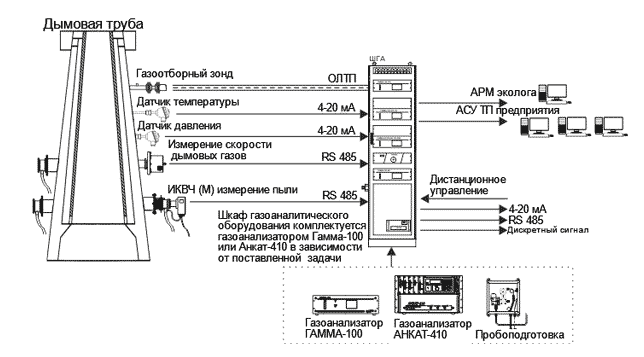
\includegraphics[width = \textwidth]{image/chapter_1/typestructure}	
		\caption{Типовая структура газоаналитической системы}
 		\label{fig:typestructure}
	\end{figure}

	Рассмотрим подробнее различные элементы схемы. Пробоотборное оборудование устанавливается непосредственно в месте отбора пробы и выполняет следующие функции:
	\begin{enumerate}[label={\arabic*)}]
		\item предварительное охлаждение;
		\item фильтрация газовой смеси;
		\item автоматическая продувка пробоотборника.
	\end{enumerate}

	Длина линии транспортирования пробы, в том числе обогреваемой, до 150 метров (для КГО на базе масс-спектрометров до 300 метров). Обогреваемая линия транспортирования пробы предназначена для переноса газовой пробы от газохода до газоанализаторов без пробоподготовки при температурах окружающей среды от -50 до +50 °C без выделения конденсата. Необогреваемая линия транспортирования пробы предназначена для переноса неочищенной газовой пробы при температуре окружающей среды от +5 до +50 °C.
	
	Устройство пробоподготовки предназначено для подготовки газовой пробы для анализа. Также выполняет задачи по удалению влаги, пыли, в том числе по автоматическому сливу конденсата, а также регулировки и стабилизации расхода пробы через газоанализатор (автоматическое переключение каналов измерения).
	
	В состав шкафа газоаналитического (далее -- ШГА) входят различные газоанализаторы, измерители и анализаторы, предназначенные для измерения компонентного состава в контролируемой газовой пробе (измерение массовой концентрации газов, пыли, температуры и скорости потока дымовых газов). К наиболее распространённым приборам, применяемым в газоаналитических системах экологического контроля, относятся
	\begin{enumerate}[label={\arabic*)}]
		\item АНКАТ-410 газоанализатор промышленных выбросов стационарный многоканальный (возможный ряд измеряемых газов (до 6 компонентов одновременно): О2, СО, СО2, NО, NО2, SО2, H2S, НCL, NН3, Cl2, СО, NО, NОХ, SСН);
		\item ГАММА-100 газоанализатор многокомпонентных смесей автоматический многофункциональный стационарный (возможный ряд измеряемых газов (до 3 компонентов одновременно): СО, СО2, SО2, H2, N2, CН4, NO, О2, He);
		\item ИКВЧ-М измеритель концентрации пыли (пылемер) оптический (по методу светопропускания) стационарный;
		\item SERVOPRO 4900 (SERVOMEX) газоанализатор промышленных выбросов стационарный многоканальный (возможный ряд измеряемых газов: О2, СО, СО2, NО, NО2, SО2, CH4).
	\end{enumerate}

	Еще одним важным элементом является автоматизированное рабочее место (АРМ) эколога (устройства сбора и передачи информации). Оно применяется при необходимости сбора и передачи информации в АСУП предприятия.
	
	На основании вышеизложенной информации можно сделать вывод о дороговизне инструментального метода мониторинга промышленных выбросов. Также можно сказать о сложности внедрения и эксплуатации подобных систем.
	
\subsection {Расчетный метод}

	Данный метод используется для расчетов рассеивания выбросов от дымовых труб, вентиляционных шахт, а также от источников организованного выброса загрязняющих атмосферный воздух веществ из установленных отверстий (далее -- от точечных источников выброса) при условии, что скорость $\omega_0$ выхода газо-воздушной смеси (далее -- ГВС) из устья источника выброса не превосходит скорости звука в атмосферном воздухе (в целях данных Методов принимается равной 330 м/с), а температура $T_\textup{г}$ ГВС не превышает 3000°С [\ref{Об утверждении методов расчетов рассеивания выбросов вредных (загрязняющих) веществ в атмосферном воздухе}].
	
	Максимальная приземная разовая концентрация загрязняющего вещества (далее -- ЗВ)  $c_M$, мг/м , при выбросе ГВС из одиночного точечного источника с круглым устьем достигается при опасной скорости ветра $u_M$ на расстоянии $x_M$ от источника выброса и определяется по формуле:
	\begin{equation}
		c_M = \frac{AMFmn\eta}{H^2\sqrt[3]{V_1\Delta T}},
		\label{eq:Cm}
	\end{equation}
	где $A$ -- коэффициент, зависящий от температурной стратификации атмосферы, определяющий условия горизонтального и вертикального рассеивания ЗВ в атмосферном воздухе;\\ 
	\hspace*{0.8cm}$M$ -- масса ЗВ, выбрасываемого в атмосферный воздух в единицу времени (мощность выброса), г/с;\\
	\hspace*{0.8cm}$F$ -- безразмерный коэффициент, учитывающий скорость оседания ЗВ в атмосферном воздухе;\\
	\hspace*{0.8cm}$m$ и $n$ -- безразмерные коэффициенты, учитывающие условия выброса из устья источника выброса;\\
	\hspace*{0.8cm}$\eta$ -- безразмерный коэффициент, учитывающий влияние рельефа местности (определяемый в соответствии с главой VII настоящих Методов);\\
	\hspace*{0.8cm}$H$ -- высота источника выброса, м;\\
	\hspace*{0.8cm}$\Delta T$ -- разность между температурой выбрасываемой ГВС $T_\textup{г}$ и температурой атмосферного воздуха $T_\textup{в}$, °С.\\
	\hspace*{0.8cm}$V_1$ -- расход ГВС, м/с, определяемый по формуле:\\
	\vspace*{-0.4cm}
	\begin{equation*}
		V_1 = \frac{\pi D^2}{4} \omega_0,
		\label{eq:V1}
	\end{equation*}
	где $D$ -- диаметр устья источника выброса, м;\\          
	\hspace*{0.8cm}$\omega_0$ -- средняя скорость выхода ГВС из устья источника выброса, м/с.
	
	Мощности $M$ выброса, высоты источников $H$, диаметры устьев $D$, температуры $T_\textup{г}$ и расходы $V_1$ ГВС при проектировании предприятий должны определяться расчетом в технологической части проекта (для проектируемых, вводимых в эксплуатацию построенных и реконструированных объектов). Для действующих производств должны определяться по результатам инвентаризации стационарных источников выбросов вредных (загрязняющих) веществ в атмосферный воздух.
	
	При расчете максимальных разовых концентраций принимаются сочетания при времени осреднения 20-30 мин значений $M$ и $V_1$, реально возможные в течение года при безаварийных условиях эксплуатации предприятия, при которых достигается максимальная концентрация $c_M$ ЗВ. Способ определения зависимости мощности выброса $M$ от скорости ветра определяется методикой расчета выбросов вредных (загрязняющих) веществ в атмосферный воздух стационарными источниками выброса.
	
	При определении величины $\Delta T$ для предприятий, работающих по сезонному графику, допускается принимать значения расчетной температуры окружающего атмосферного воздуха $T_\textup{в}$ равными средним месячным температурам воздуха за самый холодный месяц. Для остальных источников выбросов расчетная температура $T_\textup{в}$ принимается равной средней максимальной температуре воздуха наиболее теплого месяца года.
	
	Коэффициенты $m$ и $n$ определяются в зависимости от характеризующих свойства источника выброса параметров $\nu_M$, $\nu_M^\prime$, $f$ и $f_e$:
	\begin{equation*}
		\nu_M = 0,65\sqrt[3]{\frac{V_1 \Delta T}{H}},
		\label{eq:nuM}
	\end{equation*}
	\begin{equation*}
		\nu_M^\prime = 1,3\frac{\omega_0 D}{H},
		\label{eq:nuMstrih}
	\end{equation*}
\vspace*{-1.0cm}
	\begin{equation*}
		f = 1000\frac{\omega_0^2 D}{H^2 \Delta T},
		\label{eq:f}
	\end{equation*}
\vspace*{-1.1cm}
	\begin{equation*}
		f_e = 800(\nu_M^\prime)^3.
		\label{eq:fe}
		\vspace*{-0.4cm}
	\end{equation*}
	Коэффициент $m$ определяется по формуле:
	\begin{equation*}
		m = 
		\begin{dcases}
			\frac{1}{0,67+0,1\sqrt{f}+0,34\sqrt[3]{f}} \textup{, при } f < 100, \vspace*{0.4cm} \\ 
			\frac{1,47}{\sqrt[3]{f}} \textup{, при } f \geq 100.
		\end{dcases}
		\label{eq:m1}
	\end{equation*}

	Для $f_e < f < 100$ коэффициент $m$ вычисляется при $f=f_e$. Коэффициент $n$ при $f < 100$ определяется по следующей формуле:
	\begin{equation}
		n = 
		\begin{dcases}
			4,4 \nu_M \textup{, при } \nu_M < 0,5, \vspace*{0.1cm} \\ 
			0,532 \nu_M^2 - 2,13 \nu_M + 3,13 \textup{, при } 0,5 \leq \nu_M < 2, \vspace*{0.1cm} \\ 
			1 \textup{, при } \nu_M \geq 2.
		\end{dcases}
	\label{eq:n123}
	\end{equation}
	Для $f \geq 100$ (или $0~\leq~\Delta T < 0,5$) и $\nu_M^\prime = 0,5$ (холодные выбросы) при расчете $c_M$ вместо формулы~(\ref{eq:Cm}) используется формула:
	\begin{equation*}
		c_M = \frac{AMFn\eta}{H^{\frac{4}{3}}} K,
		\label{eq:Cm2}
	\end{equation*}
	где	
	\begin{equation*}
		K = \frac{D}{8V_1} = \frac{1}{7,1\sqrt{\omega_0 V_1}},
		\label{eq:K}
	\end{equation*}
	причем $n$ определяется по формуле~(\ref{eq:n123}), при $\nu_M=\nu_M^\prime$.
	
	Аналогично при $f < 100$ и $\nu_M~<~0,5$ или $f~\geq~100$ и $\nu_M^\prime~<~0,5$ (случаи предельно малых опасных скоростей ветра) расчет $c_M$ производится по формуле:
	\begin{equation}
		c_M = \frac{AMFm^\prime \eta}{H^{\frac{7}{3}}},\quad m^\prime = 
		\begin{dcases}
			2,86 m \textup{, при } \nu_M < 0,5, \vspace*{0.1cm} \\
			0,9 \textup{, при } f \geq 100 \textup{, } \nu_M^\prime < 0,5.
		\end{dcases}
		\label{eq:Cm3}
	\end{equation}

	Формула~(\ref{eq:Cm3}) при $m^\prime = 0,9$ применяется также при расчете концентраций ЗВ для источников выбросов, у которых вертикальная составляющая скорости поступающей в атмосферу газо-воздушной смеси не превышает 0,01 м/с, а давление в ней, ее плотность и температура отличаются от соответствующих характеристик атмосферного воздуха не более, чем на 0,01\% (далее -- источник выбросов фиксированной высоты) $H$ при $0 \leq \nu_M^\prime < 0,5$ и $-0,5~\leq~\Delta T~\leq~0,5$. Расстояние $x_M$ от источника выброса, на котором приземная концентрация $c$ ЗВ при неблагоприятных метеорологических условиях достигает максимального значения $c_M$, определяется по формуле:
	\begin{equation*}
		x_M = \frac{5 - F}{4} d H.
		\label{eq:Xm}
		\vspace*{-0.2cm}
	\end{equation*}

	Безразмерный коэффициент $d$ при $f<100$ находится по формуле:
	\begin{equation*}
		d = 
		\begin{dcases}
			2,48(1 + 0,28\sqrt[3]{f_e}) \textup{, при } \nu_M \leq 0,5,  \vspace*{0.1cm} \\
			4,95 \nu_M (1 + 0,28\sqrt[3]{f_e}) \textup{, при } 0,5 < \nu_M \leq 2, \vspace*{0.1cm} \\
			7 \sqrt{\nu_M}(1 + 0,28\sqrt[3]{f_e}) \textup{, при } \nu_M > 2. 
		\end{dcases}
		\label{eq:d3}
	\end{equation*}
	При $f<100$ или $0 \leq \Delta T < 0,5$ коэффициент $d$ находится по формуле):
	\begin{equation*}
		d = 
		\begin{dcases}
			5,7 \textup{, при } \nu_M^\prime \leq 0,5,  \vspace*{0.1cm} \\
			11,4 \nu_M^\prime \textup{, при } 0,5 < \nu_M^\prime \leq 2,  \vspace*{0.1cm} \\
			16 \sqrt{\nu_M^\prime} \textup{, при } \nu_M^\prime > 2.
		\end{dcases}
		\label{eq:d6}
	\end{equation*}

	Для источника выброса фиксированной высоты $H$ при $0~\leq~\nu_M^\prime < 0,5$ и $-0,5~\leq~\Delta T \leq 0$ значение $x_M$ принимается равным $5,7H$.
	
	Опасная скорость ветра $u_M$ на стандартном уровне флюгера (10 м от уровня земли), при которой достигается наибольшая приземная концентрация ЗВ $c_M$, в случае $f~<~100$ определяется по формуле:
	\begin{equation*}
		u_M = 
		\begin{dcases}
			0,5  \textup{, при } \nu_M \leq 0,5,  \vspace*{0.1cm} \\
			\nu_M \textup{, при } 0,5 < \nu_M \leq 2, \vspace*{0.1cm} \\
			\nu_M(1 + 0,12\sqrt{f}) \textup{, при } \nu_M > 2.
		\end{dcases}
		\label{eq:uM3}
	\end{equation*}
	При $f<100$ или $0 \leq \Delta T < 0,5$ значение $u_M$ вычисляется по формуле:
	\begin{equation*}
		u_M = 
		\begin{dcases}
			0,5  \textup{ при } \nu_M^\prime \leq 0,5, \vspace*{0.1cm} \\
			\nu_M^\prime \textup{ при } 0,5 < \nu_M^\prime \leq 2, \vspace*{0.1cm} \\
			2,2 \nu_M^\prime \textup{ при } \nu_M^\prime > 2.
		\end{dcases}
		\label{eq:uM6}
	\end{equation*}
	Для источника выброса фиксированной высоты $H$ при $0 \leq \nu_M^\prime < 0,5$ и $-0,5 \leq \Delta T \leq 0$ принимается $u_M = 0,5$ м/с.

	Описанный выше расчетный метод контроля выбросов имеет множество плюсов, главным из которых является меньшие затраты на установку и содержание оборудования. К минусам данного метода можно отнести низкую точность получаемых результатов при недостатке данных для расчетов. При этом нельзя сказать, что расчетный метод полностью не зависит от технически сложных устройств, так как для расчетов необходимы многие характеристики выбросов, что значительно снижает его эффективность.
	
\section [\vspace*{-0.22cm}Применение тепловизоров для контроля выбросов загрязняющих \hspace*{-0.9cm} веществ в атмосферу]{\vspace*{-0.22cm}Применение тепловизоров для контроля выбросов загрязняющих \\ \hspace*{-2.25cm} веществ в атмосферу}
\subsection{Тепловизоры и области их применения}
	Тепловизоры -- устройства, предназначенные для наблюдения нагретых объектов по их собственному тепловому излучению. Они преобразуют невидимое глазом человека инфракрасное излучение в электрические сигналы, которые после усиления и автоматической обработки вновь преобразуются в видимое изображение объектов [\ref{Тепловизоры: справочник}].
	
	Различают несколько классификацийданных устройств. По принципу получения изображения тепловизоры делятся на:
	\begin{enumerate}[label={\arabic*)}]
		\item тепловизоры с оптико-механическим сканированием. Основные элементы тепловизоров с оптико-механическим сканированием;
		\item матричные тепловизоры.
	\end{enumerate}	

	Для получения видимого изображения теплоизлучающего объекта в тепловизорах с оптико-механическим сканированием осуществляют разложение (развертку) объекта на некоторое число элементарных площадок. Каждая такая площадка, называемая элементом разложения, является наименьшей деталью, которую может воспроизвести данная система. Анализ мощности теплового излучения отдельных элементов производится приемником излучения, с выхода которого последовательно во времени снимаются сигналы, содержащие информацию о теплоизлучающем объекте и окружающем его фоне. Таким образом, двумерное распределение яркостей в пространстве объектов в результате сканирования преобразуется в одномерное распределение напряжения на нагрузочном резисторе приемника излучения. Сигналы с приемника передаются по одному каналу в индикатор видео устройства (Видеоконтрольное устройство), который преобразует их в видимое изображение. Чаще всего в качестве индикатора ВКУ используют электронно-лучевую трубку (кинескоп). Так как в каждый момент времени на экране кинескопа воспроизводится только один элемент изображения, закон движения электронного луча кинескопа должен быть идентичен закону развертки, что достигается применением синхронизирующих элементов.
	
	Одним из главных элементов тепловизоров с оптико-механическим сканированием, определяющим их температурную чувствительность и максимальную дальность действия, является приемник инфракрасного излучения. Чувствительные элементы приемников представляют собой фото-резисторы, проводимость которых изменяется под действием падающего на излучения. Главным параметром приемников инфракрасного излучения является порог чувствительности -- минимальный поток излучения, который вызывает на выходе приемника сигнал, равный напряжению шумов, или превышающий его в заданное число раз.
	
	В техническом отношении одним из преимуществ таких тепловизоров является то, что они построены на основе матричного инфракрасного детектора. Это преимущество проявляется в сравнении с тепловизорами, использующими сканирующие системы, и которых много ещё на мировом рынке. В связи с использованием принципа накопления информационного сигнала матричные тепловизоры при прочих равных условиях выигрывают у сканирующих систем по совокупности таких параметров, как надёжность, чувствительность, быстродействие и пространственное разрешение. Типовая блок-схема матричных тепловизоров приведена на рисунке~\ref{fig:MatrixIRCameraScheme} [\ref{Основы тепловидения: учебное пособие}].
	
	\begin{figure}[h!]
		\centering
		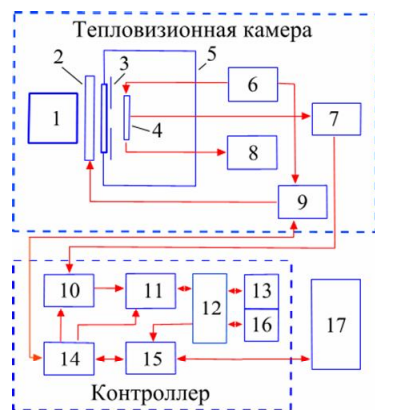
\includegraphics[width = \textwidth]{image/chapter_1/MatrixIRCameraScheme}	
		\caption{Блок-схема тепловизионной камеры: 1 -- объектив;\\2 -- устройство калибровки; 3 -- холодная диафрагма;\\4 -- матричное ФПУ; 5 -- вакуумный криостат с просветленным окном;\\6 -- генератор управляющих импульсных и постоянных напряжений;\\7 -- усилитель с дифференциальным выходом; 8 -- измеритель температуры ФПУ и автомат включения напряжения смещения подложки из InAs; 9,14 -- блоки управления и синхронизации;\\10 -- АЦП; 11 -- сумматор; 12 -- диспетчер памяти; 13,16 -- банки памяти;\\15 -- блок связи с персональным компьютером; 17 -- персональный компьютер}
		\label{fig:MatrixIRCameraScheme}
	\end{figure}

	На сегодняшний день известно множество способов применения тепловизоров. Один из них -- получение информации о состоянии материалов, степени их износа, примером является контроль за состоянием облицовки доменных печей. Полная замена облицовки доменных печей является весьма дорогой процедурой, так как влечет остановку производства на 3-4 дня. Использование тепловизора позволит быстро обнаружить трещины и иные повреждения [\ref{Тепловизионные системы в исследовании тепловых процессов}].
	
	Помимо применения в дефектоскопии тепловизионные устройства широко применяются для снятия тепловых карт местности. Этот способ основан на дистанционном измерении температуры земной поверхности с самолета или с искусственного спутника земли. Тепловые карты позволяют судить о геологическом строении и полях активности кратеров, способствуют поискам и регистрации тепловых источников, гейзеров, мест подземных утечек в энергосистемах, тепломагистралях, дренажных устройствах, позволяет своевременно обнаруживать очаги зарождающихся пожаров и определять границы крупных пожаров сквозь пелену сплошного дыма, а также границы пожаров горючих ископаемых по скрытым очагам в штабелях угля, сланцев, шахтных отвалов и т. д.
	
	Еще одной областью в которой тепловизоры нашли широкое применение является медицина [\ref{Использование Тепловизора в комплексной
		диагностике и лечении заболеваний опорно-двигательной системы}]. Тепловидение или термография значительно расширяет обычные области применения инфракрасной техники в медицине, так как позволяет не только фотографировать освещенную инфракрасными лучами поверхность тела человека и расположенные вблизи от нее сосуды, но и наблюдать изображения, создаваемые собственным тепловым излучением тела. Тепловидение является хотя и эффективным, но дополнительным методом при диагностике различных заболеваний; полезно сочетание тепловизионного метода исследования с другими, например, рентгенологическим, ультразвуковым, радиоизотопным, лазерным, охватывающими более широкий спектр электромагнитных волн.
	
\subsection{Применение тепловизоров для решения смежных проблем}
	На сегодняшний день тепловизоры часто применяются также для решения проблем, смежных поставленной нами задачи контроля за выбросами вредных веществ в атмосферу на промышленных предприятиях [\ref{triplepundit.com}]. Примером такой проблемы является контроль за факелом газа сжигаемого на нефтехимических заводах. Использование теплвизоров обеспечивает надежный контроль за температурой пламени факела, его объемом и формой. Преимуществом тепловизоров перед оптическими видеосистемами является не зависимость от времени суток и погодных условий. Тепловизоры также выгодно отличаются от других систем контроля температуры, так как могут контролировать процесс с безопасного расстояния, что позволяет сэкономить на системах защиты тепловизора. Схематичное устройство системы представлено на рисунке~\ref{fig:controlGasSystem} [\ref{Early fire detection and condition monitoring}].
	
	\begin{figure}[ht!]
		\centering
		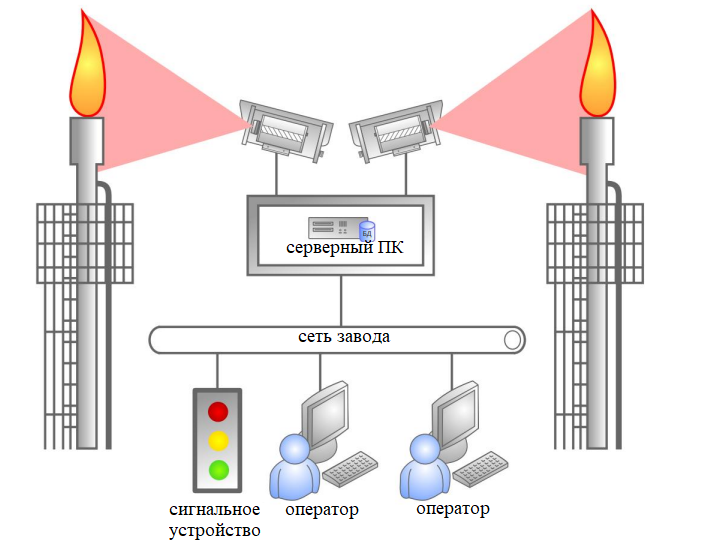
\includegraphics[width = 13cm]{image/chapter_1/controlGasSystem}	
		\caption{Схематичное устройство системы\\контроля за факелом горения газа}
		\label{fig:controlGasSystem}
	\end{figure}

	Помимо этого есть другой пример использования тепловизоров для обнаружения газовоздушных смесей. Компания FLIR провела исследование использования тепловизоров для обнаружения выбросов, производимых автомобилями, и получила интересные результаты [\ref{Gasoline and diesel passenger car emissions deterioration using on-road emission measurements and measured mileage}]. В исследовании было продемонстрировано движение автомобилей, снятое тепло-видео системой наблюдения. На оптическом видео различить выбросы не представлялось возможным, тогда как в инфракрасном спектре был отчетливо виден факел выхлопных газов автомобиля. В результате этого исследования было обнаружено, что тепловизоры способны обнаруживать даже невидимые невооруженным глазом вредные выбросы. Это говорит о том, что тепловизоры можно использовать  для контроля за любым видом выбросов, в том числе неразличимых в оптическом спектре. 
	
\section{Выводы по главе 1}
	В данной главе были рассмотрены современные способы контроля вредных выбросов. Были рассмотрены инструментальный и расчетный методы. Также были рассмотрены современные области применения тепловизоров.
	
	Инструментальный метод основан на использовании сложного оборудования -- газоанализаторов и является наиболее точным способом контроля за выбросами вредных предприятий, позволяет получить подробную статистику по всем веществам, которые выбрасываются в атмосферу данным предприятием. Однако, эта точность компенсируется очень высокой стоимостью эксплуатации, сложностью установки и подключения. 
	
	Расчетный метод основан на использовании формул для расчетов концентраций вредных веществ в атмосфере. Этот метод является менее точным, однако затраты на оборудование существенно сокращаются.
	
	В качестве решения этой проблемы были рассмотрены тепловизоры. Для более эффективного и точного анализа необходимо иметь возможность получать сегментированное изображение факела вредных выбросов. В результате исследования современных областей применения тепло-видео систем наблюдения было обнаружено, что тепловизоры способны обнаруживать даже не видимые в оптическом спектре нагретые газо-воздушные смеси. Это позволит существенно увеличить точность работы расчетного метода, при этом еще больше сократив расходы на оборудование. Таким образом имеет смысл разработать программный комплекс осуществляющий сегментацию факела выбросов с использованием тепло-видео систем наблюдения.
	
\chapter[\vspace*{-0.22cm}СЕГМЕНТАЦИЯ ФАКЕЛА ВЫБРОСОВ С ПОМОЩЬЮ \\ \hspace*{-0.35cm}ТЕПЛОВЫХ СНИМКОВ]{\vspace*{-0.22cm}СЕГМЕНТАЦИЯ ФАКЕЛА ВЫБРОСОВ С ПОМОЩЬЮ ТЕПЛОВЫХ СНИМКОВ}
\section{Постановка задачи сегментации факела выбросов}

	Необходимо провести классификацию пикселей последовательности изображении и соответствующих им элементов последовательности матриц температур, представляющих оптический и тепловой видео потоки, полученные с тепло-видео системы наблюдения. Выделить необходимо два класса -- области соответствующие факелу вредных выбросов предприятий и не принадлежащие факелу. Если выражаться более формальным языком, определим целевую функцию~(\ref{eq:segment_func}), которая задает отображение множества $X$ на множество $Z$.
	\vspace*{-0.2cm}
	\begin{equation}
		f: X \rightarrow Z,
		\label{eq:segment_func}
		\vspace*{-0.4cm}
	\end{equation}
	где X -- множество последовательностей из пар вида $x_i, y_i$, где $x_i$ -- элемент множества изображений в пространстве RGB, представленных трехмерной матрицей, $y_i$ -- элемент множества двухмерных матриц, состоящих из чисел от 0 до 255. $Z$ - множество последовательностей двухмерных матриц состоящих из вещественных чисел в диапазоне от 0 до 1, обозначающих вероятность принадлежности соответствующей пары пикселя и температуры к факелу вредных выбросов (маска).
	
	Для того, чтобы восстановить целевую функцию~(\ref{eq:segment_func}) необходимо разработать алгоритм $A$, $A: X \rightarrow Z$. Этот алгоритм должен соответствовать следующим требованиям:
	\begin{enumerate}[label={\arabic*)}]
		\item должен для некоторых элементов множества $X$, составляющих тестовую выборку находить маски максимально точно соответствующие заранее полученным элементам множества $Z$;
		\item должен приближать целевую функцию для всех элементов из множества $X$;
		\item должен допускать численную реализацию;
		\item должен обеспечивать связность области дыма на маске.
	\end{enumerate}

\section{Подготовка данных}
\subsection{Работа с тепловизором}

	Для решения поставленной задачи необходимо разработать алгоритм взаимодействия с тепловизором и научиться получать данные для последующей обработки. Для выполнения задачи был выбран тепловизор модели DS60xxFT-M (см.~рисунок~\ref{fig:teploviser}). Данное устройство предоставляет возможность получения оптических снимков в разрешении 1920 на 1080 пикселей, с частотой развертки в 25 Гц, а также тепловые снимки в разрешении 640 на 512 пикселей, с частотой в 25 Гц. Для данной модели тепловизора была разработана SDK (Software Development Kit -- комплект для разработки программного обеспечения). Данный комплект инструментов представляет из себя набор готовых программ для подключения к тепловизору с персонального компьютера, а также взаимодействия с тепловизором. В перечень возможностей данного набора программ входит:
	
	\begin{enumerate}[label={\arabic*)}]
		\item дистанционное упраление углом наклона и поворота тепловизора;
		\item изменение уровня увеличения оптической камеры;
		\item включение и выключение подсветки;
		\item получение потока оптических снимков;
		\item получение потока тепловых снимков;
		\item получение матрицы температур;
		\item сохранение оптических и тепловых снимков покадрово в память компьютера.
	\end{enumerate}

	\begin{figure}[h!]
		\centering
		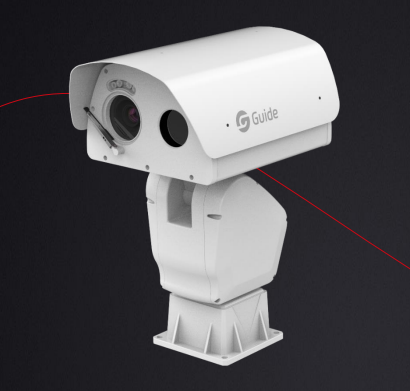
\includegraphics[width = 13cm]{image/chapter_2/teploviser}	
		\caption{Тепловизор выбранной модели}
		\label{fig:teploviser}
	\end{figure}

	Все программы предоставляются в виде исходного кода с возможностью редактирования. Помимо SDK, предоставляется библиотека для работы с тепловизором и документация, используя которые можно самостоятельно разрабатывать программное обеспечения с необходимым функционалом или же модифицировать уже имеющиеся в SDK программы.

	Ввиду ограниченности возможностей библиотеки, запись возможна только в формате YUV [\ref{Understanding color models: a review}], который является цветовой моделью, в которой цвет состоит из трёх компонентов — яркость ($Y$) и два цветоразностных компонента ($U$ и $V$). Компоненты YUV определены на основе компонент RGB~следующим~образом:
	\vspace*{-0.4cm}
	\begin{equation*}
		Y = K_R R + (1 - K_R - K_B)G + K_B B,
		\label{eq:Y_in_YUV}
	\end{equation*}
\vspace*{-1.3cm}
	\begin{equation*}
		U = B - Y,
		\label{eq:U_in_YUV}
	\end{equation*}
\vspace*{-1.5cm}
	\begin{equation*}
		V = R - Y.
		\label{eq:V_in_YUV}
		\vspace*{-0.4cm}
	\end{equation*}
	
	Также возможно обратное преобразование в RGB. Оно производится по формулам:
	\begin{equation*}
		R = Y + V,
		\label{eq:R_in_YUV}
	\end{equation*}
\vspace*{-1.2cm}
	\begin{equation*}
		G = Y - \frac{K_R V + K_B U}{1 - K_R - K_B},
		\label{eq:G_in_YUV}
	\end{equation*}
\vspace*{-1.2cm}
	\begin{equation*}
		B = Y + U.
		\label{eq:B_in_YUV}
		\vspace*{-0.4cm}
	\end{equation*}
	где $K_R=0.2126$ и $K_B=0.0722$ -- константы. $R$, $G$, $B$ -- компоненты модели RGB, обозначающие интенсивность красного, синего и зеленого цветов.

\subsection{Преобразование цветовой карты}
	
	Следующей подзадачей, которую необходимо решить, является преобразование цветовой карты тепловых снимков. Цветовая карта -- это некоторая функция
	\vspace*{-0.4cm}
	\begin{equation}
		f: X \rightarrow Y,
		\label{eq:fXY}
		\vspace*{-0.4cm}	
	\end{equation}
	 где $X$ -- интенсивность пикселя в оттенках серого, $Y$ -- вектор, обозначающий цвет пикселя в пространстве RGB [\ref{Diverging Color Maps for Scientific Visualization (Expanded)}]. Зачастую полученные таким образом изображения являются более наглядными, чем изображения в оттенках серого. Для тепловых снимков традиционно применяется цветовая карта <<JET>> (рисунок~\ref{fig:opt_example}). 
	
	\begin{figure}[ht!]
		\centering
		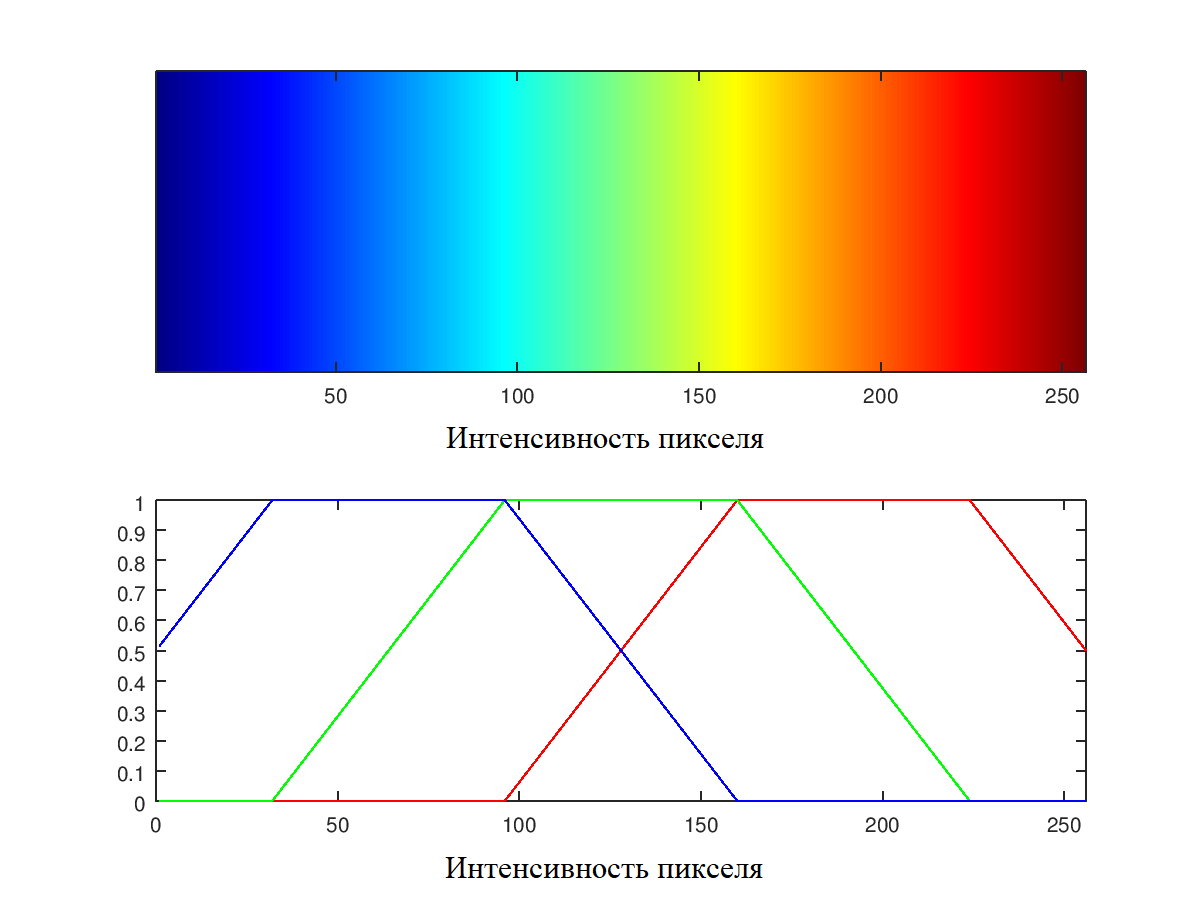
\includegraphics[width = 13cm]{image/chapter_2/jet}	
		\caption{График преобразования цвета в\\цветовой карте <<JET>>}
		\label{fig:jet}
	\end{figure}
	
	В разработанной системе тепловые снимки также сохраняются в цветовой карте <<JET>>. Для поставленной задачи необходимо разработать алгоритм для преобразования изображение к оттенкам серого (рисунок~\ref{fig:gray_tep_example}). Ввиду технических особенностей как тепловые, так и оптические снимки передаются в закодированном формате JPEG, что приводит к искажению цветов. Другой помехой к прямой конвертации в оттенки серого является отсутствие общего стандарта для конвертации изображения, из-за чего функция может незначительно отличаться. Все это приводит к невозможности задания обратной функции 
	\vspace*{-0.2cm}
	\begin{equation}
		g: Y \rightarrow X
		\label{eq:gYX}
		\vspace*{-0.4cm}
	\end{equation}
	для конвертации из цветовой карты в оттенки серого аналитическим путем. 
	\begin{figure}[h!]
		\begin{subfigure}{.45\textwidth}
			\centering
			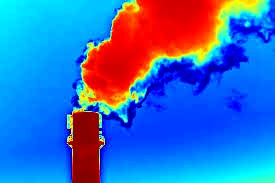
\includegraphics[width = \textwidth]{image/chapter_2/abstrtact_JET_example}
			\caption{}
		\end{subfigure}
		\begin{subfigure}{.45\textwidth}
			\centering
			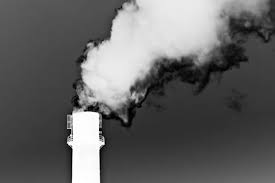
\includegraphics[width = \textwidth]{image/chapter_2/abstrtact_gray_example}
			\caption{}
		\end{subfigure}
		\centering
		\caption{Пример теплового снимка приведенного к оттенкам \\серого: a) изображение в цветовой карте <<JET>>; б) изображение в оттенках серого}
		\label{fig:gray_tep_example}
	\end{figure}

	В общем случае для решения поставленной задачи необходимо решить следующую подзадачу. Необходимо сопоставить каждому цвету из пространства RGB некоторую интенсивность пикселя, выполнив классификацию. Более формальным языком, $Y$ -- множество одномерных векторов длины 3 вида $[r_i, g_i, b_i]$, где $r_i, g_i, b_i$ -- целые числа от 0 до 255, $X$ -- множество целых чисел от 0 до 255. Необходимо восстановить целевую функцию~(\ref{eq:gYX}) и реализовать для этого алгоритм отвечающий следующим требованиям:
	\begin{enumerate}[label={\arabic*)}]
		\item для векторов полученых в результате преобразовании с помощью функции~(\ref{eq:fXY}), должен находить значение, максимально приближенное к обратному преобразованию;
		\item для векторов из $Y$, не являющихся результатом функции~(\ref{eq:fXY}), должен также приближать целевую функцию;
		\item должен допускать численную реализацию.
	\end{enumerate}
	
	Для восстановления функции $g$ было решено использовать модель машинного обучения <<FlannBasedMatcher>> [\ref{OpenCV: Feature Detection and Description}], которая в общем случае позволяет задать отображение
	\vspace*{-0.2cm}
	\begin{equation}
		h: A \rightarrow B_i,
		\label{eq:hABi}
		\vspace*{-0.4cm}
	\end{equation}
	где $A$ -- некоторая трехмерная матрица фиксированных размеров, $B$ -- пространство трехмерных матриц такой же размерности. Введем оценку расстояния между трехмерными матрицами, которая будем вычислять по формуле~(\ref{eq:D(A,B)}).
	\begin{equation}
		D(A, B) = \sqrt{\sum\limits_{i=1}^n \sum\limits_{j=1}^m \sum\limits_{k=1}^p (A_{ijk} - B_{ijk})^2},
		\label{eq:D(A,B)}
	\end{equation}
	где $n, m, p$ - размерности матриц. При этом для отображения~(\ref{eq:hABi}) имеем 
	\vspace*{-0.2cm}
	\begin{equation*}
		D(A, B_i) = min(D(A, B_j)), 
		\label{eq:D(A,B_i)}
		\vspace*{-0.4cm}
	\end{equation*}
	где $j~\in~[0, n-1]$, $n$ -- количество трехмерных матриц в пространстве $B$. 
	
	Данная модель основана на методе $k$ ближайших соседей [\ref{k-Nearest neighbour classifiers: a tutorial}]. $k$ ближайших соседей -- непараметрический метод классического машинного обучения с учителем, использующийся для решения задач классификации и регрессии. 
	
	Рассмотрим решение задачи классификации данным методом подробнее. В общем виде необходимо восстановить целевую функцию вида:
	\vspace*{-0.5cm}
	\begin{equation*}
		f: X \rightarrow Y, 
		\label{KNNf}
		\vspace*{-0.5cm}
	\end{equation*}
	где $X$ -- множество векторов признаков, каждый из которых является некоторой численной величиной, $Y$ -- множество классов, каждый класс является некоторой дискретной величиной. Для обучения используется обучающая выборка, которая представляет из себя множество пар $x_i$ и $y_i$, где $x_i~\in~X$, а $y_i~\in~Y$.
	Алгоритм классификации некоторого вектора признаков $x_0$ в общем случае состоит из трех шагов:
	\begin{enumerate}[label={\arabic*)}]
		\item для каждой пары $x_i$, $y_i$ вычисляется расстояние $d_i$
		\begin{equation*}
			d_i = \sqrt{\sum\limits_{j=1}^n (x_{ij} - x_{0j})^2}, 
			\label{disqrt}
		\end{equation*}
		где $n$ - количество признаков;
		\item выбирается некоторая последовательность $a$ индексов $a_q$, где \linebreak $q~\in~[1, k]$, для каждого $q$ справедливо следующее неравенство $d_{a_q}~\le~d_{i}$, где $i~\notin~a$;
		\item из классов, принадлежащих последовательности $y_{a_q}$ выбирается наиболее часто встречающийся класс.
	\end{enumerate}

	При этом заметим, что если в обучающей выборке каждому классу соответствует ровно 1 вектор признаков, то имеет смысл находить ровно одного самого ближайшего соседа.
	В этом случае работу алгоритма можно существенно оптимизировать, используя метод $k$-мерного дерева.
	
	$k$-мерное дерево -- статическая структура данных для хранения точек в $k$-мерном пространстве, представляющая из себя бинарное дерево [\ref{k-мерное дерево на сайте итмо}]. Позволяет отвечать на многие запросы, например какие точки лежат в данном прямоугольнике или какая точка является ближайшей к данной. Рассмотрим алгоритм построения дерева для некоторого множества точек $x_i$ и некоторго числа $j~\in~[1, k]$:
	\begin{enumerate}[label={\arabic*)}]
		\item для упорядоченной последовательности $b$, где $b_i~=~x_{ij}$ найдем медиану $m$;
		\item разобъем множество $x_i$ на 2 подмножества $c$ и $d$, где для $\forall x_i~\in~c$ выполняется $b_i~<~m$ и для $\forall x_i~\in~d$ выполняется $b_i~\ge~m$;
		\item если точек в множестве $x$ больше двух, то для правого поддерева вызовем рекурсивно алгоритм для множества $c$, а для левого используем множество $d$, численный параметр вычислим $j_{n}=(j + 1)~mod~k$. 
	\end{enumerate}
	 Построенное k-мерное дерево для случая двумерных точек показано на рисунке~\ref{fig:kdtreeexample}, где $p_i$ -- листья дерева содержащие 1 точку, $j_j$ -- внутренние узлы дерева.
	
	\begin{figure}[h!]
		\centering
		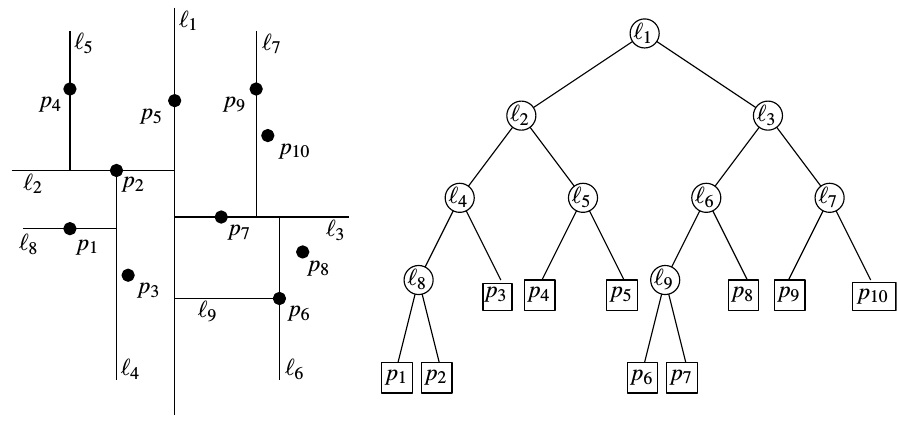
\includegraphics[width = 13cm]{image/chapter_2/kdtreeexample}	
		\caption{Пример построения k-мерного дерева}
		\label{fig:kdtreeexample}
	\end{figure}
	
	Алгоритм поиска ближайшего соседа в дереве представлен на рисунке~\ref{fig:kdtreealgo}, функция find() принимает параметром номер текущего узла. Пусть номер текущего узла -- $v$, тогда номер левого и правого потомков равны $2v$ и $2v~+~1$ соответственно.
	
	\begin{figure}[h!]
		\centering
		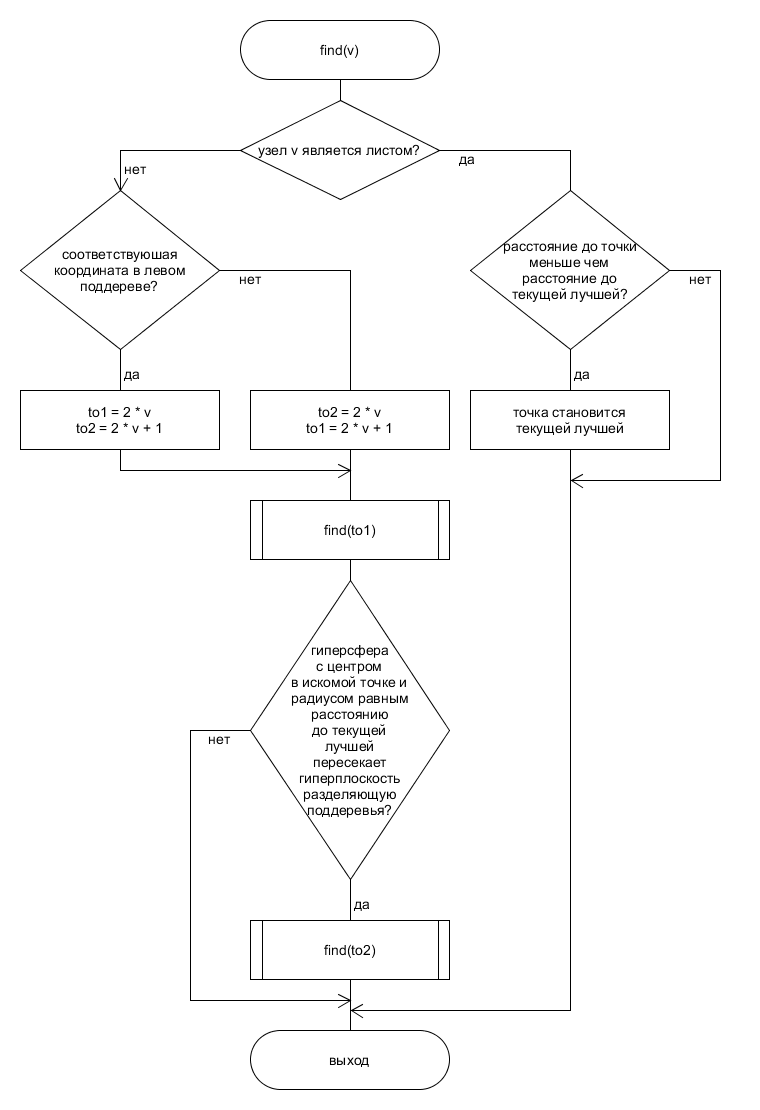
\includegraphics[width = 0.9\textwidth]{image/chapter_2/kdtreealgo}	
		\caption{Схема алгоритма поиска ближайшего соседа в \\ дереве из вершины v}
		\label{fig:kdtreealgo}
	\end{figure}
	
	Для обучения данной модели была сгенерирована обучающая \\ выборка, представляющая из себя множество векторов $C^{jet}$, где $C^{jet}_{i}$ -- определяется по формуле:
	\vspace*{-0.3cm}
	\begin{equation}
		C^{jet}_{i} = f(C^{gray}_{i}),
		\label{eq:Cjetgray}
		\vspace*{-0.35cm}
	\end{equation}
	где $C^{gray}_{i}$ -- элемент $C^{gray}$ -- множества чисел от 0 до 255. С помощью полученной модели были рассчитаны значения функции $g$ для всего пространства RGB, что позволило существенно сократить время работы программы, по сути сведя функцию $g$ к обращению к трехмерной матрице. Пример результата использования функции $g$ представлен выше (см. рисунок~\ref{fig:gray_tep_example}).
	
\subsection[\vspace*{-0.22cm}Наложение карты абсолютных температур на оптические \\ \hspace*{-1.15cm}снимки]{\vspace*{-0.22cm}Наложение карты абсолютных температур на \\ \hspace*{-3.75cm}оптические снимки}	
	Заключительным этапом подготовки данных является преобразование изображения в оттенках серого в матрицу абсолютных температур и наложение полученной матрицы на оптический снимок. Изображение в оттенках серого является двумерной матрицей $A$, с высотой $h$ и длинной $w$. Элементом массива является число от 0 до 255, которое является нормированным значением температуры.
	Перед восстановлением абсолютных температур необходимо провести изменение размера матрицы относительных температур, для корректного сопоставления. Для этого воспользуемся методом билинейной интерполяции. Данный метод представляет из себя обобщение линейной интерполяции одной переменной для функций двух переменных. Функция билинейной интерполяции интерполирует значения исходной функции двух переменных в произвольной подматрице по четырём её значениям в угловых элементах подматрицы и экстраполирует функцию на всю остальную поверхность. Данная функция имеет вид: 
%	Bilinear_interpolation
	\begin{equation}
		F(x,y)=b_{1}+b_{2} x+b_{3} y+b_{4} x y,
		\label{eq:interpol}
	\end{equation}
	где $x$ и $y$ - координаты элемента матрицы; $b_1$, $b_2$, $b_3$ и $b_4$ -- некоторые неизвестные коэффициенты. Необходимо найти значение этих коэффициентов. Приведем один из способов вычисления этих коэффициентов. Для этого подставим в уравнение~\ref{eq:interpol} координаты и значения угловых 
	элементов подматрицы. Тогда необходимо решить систему из четырех уравнений~(\ref{eq:system_interpol}):
	
	\begin{equation}
	\begin{cases}
		f(Q_{11})=b_{1}+b_{2} x_{1}+b_{3} y_{1}+b_{4} x_{1} y_{1}, \\
		f(Q_{12})=b_{1}+b_{2} x_{1}+b_{3} y_{2}+b_{4} x_{1} y_{2}, \\
		f(Q_{21})=b_{1}+b_{2} x_{2}+b_{3} y_{1}+b_{4} x_{2} y_{1}, \\
		f(Q_{22})=b_{1}+b_{2} x_{2}+b_{3} y_{2}+b_{4} x_{2} y_{2}.
	\end{cases}
	\label{eq:system_interpol}
	\end{equation}
	В системе~(\ref{eq:system_interpol}) $Q_{11}$, $Q_{12}$, $Q_{21}$ и $Q_{22}$ -- угловые элементы подматрицы. Пример можно увидеть на рисунке~\ref{fig:Bilinear_interpolation}.
	\begin{figure}[h!]
		\centering
		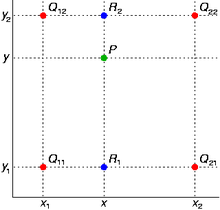
\includegraphics[width = 0.6\textwidth]{image/chapter_2/Bilinear_interpolation}	
		\caption{Пример расположения угловых точек \\при билинейной интерполяции}
		\label{fig:Bilinear_interpolation}
	\end{figure}
	Для того чтобы восстановить абсолютные температуры $T_{abs}$ воспользуемся следующей формулой:
	\begin{equation*}
		T_{abs} = T_{min} + \frac{T_{norm}(T_{max} - T_{min})}{255},
		\label{eq:T_abs}
	\end{equation*}
	где $T_{norm}$ -- нормированная температура, $T_{min}$ -- минимальная температура, $T_{max}$ -- максимальная температура. Применяя данное преобразование к каждому элементу матрицы нормированных температур получим матрицу абсолютных температур.
	
	Следующим важным этапом является процесс наложения матрицы абсолютных температур на оптический снимок. Ввиду достаточного удаления от наблюдаемого объекта становится возможным простое наложение матрицы на соответствующую область оптического снимка, без необходимости применения аффинных преобразований. 
	Для этого находим пару чисел $A, B$ -- координаты элемента с индексами $0, 0$ в матрице температур на оптическом снимке и формируем из оптического снимка $X$ новый оптический снимок $Y$, где
	\vspace*{-0.3cm}
	\begin{equation*}
		Y_{i,j} = X_{i + A,j + B},
		\label{eq:nalozhenie}
		\vspace*{-0.3cm}
	\end{equation*}
	где $i \in [0, n]$, $j \in [0, m]$, $n$ и $m$ -- размеры матрицы температур. После этого получаем пару -- изображение в формате RGB с и матрица абсолютных температур. Изображение и матрица имеют соответствующие размеры $w$ и $h$. В результате получаем данные в формате, указанном в постановке задачи. Пример наложения снимка с примененной цветовой картой показан на рисунке~\ref{fig:nalozhenie_examp}.
	\begin{figure}[h!]
		\centering
		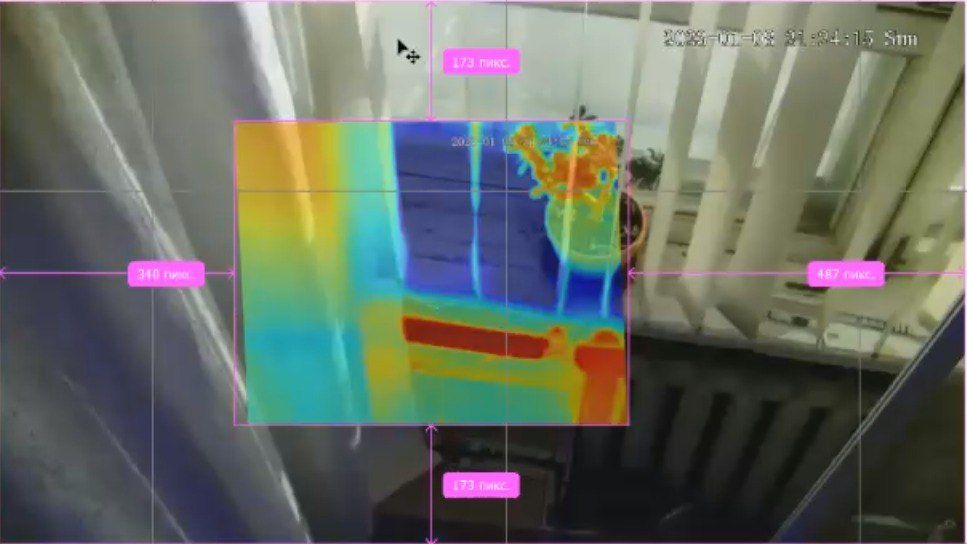
\includegraphics[width = 0.9\textwidth]{image/chapter_2/nalozhenie_examp}	
		\caption{Пример работы оптического и теплового снимков}
		\label{fig:nalozhenie_examp}
	\end{figure}
\section[\vspace*{-0.22cm}Решение задачи сегментации факела выбросов с помощью \\ \hspace*{-0.75cm}оптических и тепловых снимков]{\vspace*{-0.22cm}Решение задачи сегментации факела выбросов с помощью \\ \hspace*{-2.05cm}оптических и тепловых снимков}
\subsection{Задача детекции трубы}
	Детекция трубы как источника выбросов является необходимой для решения задачи сегментации факела выбросов на изображении по следующим причинам:
	\begin{enumerate}[label={\arabic*)}]
		\item нам необходимо выявить связную область факела выбросов, поэтому детекция трубы позволяет определить место, откуда исходят выбросы, это помогает локализовать область, где нужно искать факел выбросов на изображении;
		\item наличие трубы на изображении может приводить к ложным срабатываниям в алгоритмах, опирающихся на температуру, так как труба часто имеет сравнимую с факелом выбросов температуру, следовательно необходимо знать где находится труба, чтобы исключить ее из итоговой маски;
		\item детекция трубы может помочь в определении характеристик вредных выбросов; 
		\item детекция трубы может помочь в определении необходимой температуры для отсечения. 
	\end{enumerate}
	Таким образом, детекция трубы является важным шагом в решении задачи сегментации дыма на изображении, который помогает улучшить качество сегментации.
	
	При этом ввиду необходимости установки тепловизора, т.е. проведения некоторых подготовительных мероприятий, имеется возможность заранее определить внешний вид трубы и использовать этот образец для детекции. Задача детекции трубы на изображении заключается в определении наличия трубы на изображении и определении ее положения и размера. Сформулируем постановку задачи детекции трубы более формальным языком.
	
	Целевая функция задает отображение вида
	\vspace*{-0.2cm}
	\begin{equation}
		f : X \rightarrow Y,
		\label{f:x->[4]}
		\vspace*{-0.4cm}
	\end{equation}
	где $X$ -- множество пар вида $x_i, y_i$, где $x_i$ -- элемент множества изображений в пространстве RGB, представленных трехмерной матрицей, $y_i$ -- элемент множества двухмерных матриц, состоящих из чисел от 0 до 255. $Y$ - множество векторов $[a, b, c, d]$, содержащих координаты прямоугольника ограничивающего трубу. 
	
	Необходимо разработать алгоритм $B$, восстанавливающий целевую функцию~(\ref{f:x->[4]}), принимающий на вход пару из изображения и матрицы, а также изображение $C$ - образец трубы, и возвращающий вектор $[a, b, c, d]$. Алгоритм должен отвечать следующим требованиям:
	\begin{enumerate}[label={\arabic*)}]
		\item для изображений, содержащих трубу, должен находить значение, максимально приближенное к действительному;
		\item для содержащих часть трубы, должен также приближать целевую функцию;
		\item должен допускать численную реализацию.
	\end{enumerate}
	
	При разработке алгоритма стоит также учесть некоторые особенности. К ним можно отнести:
	\begin{enumerate}[label={\arabic*)}]
		\item смена дня и ночи, вследствие чего цвет трубы может существенно изменится;
		\item масштабируемость, изменение размеров трубы;
		\item неполнота трубы, часть трубы, которая есть на образце, может отсутствовать.
	\end{enumerate}
	Ввиду этих особенностей, был выбран алгоритм использующий вторую производную для поиска ключевых точек. Имея некоторое количество ключевых точек, можно восстановить прямоугольник, включающий трубу.\linebreak В качестве алгоритма поиска ключевых точек был выбран алгоритм <<SIFT>>
	
	Метод SIFT (Scale-Invariant Feature Transform или Масштабно-\linebreak инвариантное преобразование особенностей) - это один из наиболее популярных алгоритмов детектирования особых точек в изображениях [\ref{Scholarpedia: Scale Invariant Feature Transform}]. Основная идея метода SIFT заключается в поиске особых точек, которые инвариантны к масштабу и повороту изображения, а также устойчивы к изменениям освещения и частичной закрытости. Алгоритм SIFT состоит из нескольких этапов:
	\begin{enumerate}[label={\arabic*)}]
	\item построение пирамиды изображений: Изначальное изображение размывается с помощью гауссового фильтра с разными масштабами $G\left(x,y,k_i\sigma \right)$ в масштабе $k_i\sigma$, получаем изображение 
	\vspace*{-0.2cm}
	\begin{equation*}
		L\left(x,y,k_i\sigma \right)=G\left(k_i\sigma \right)*I\left(x,y\right), 
		\label{L(x,y,sigma)}
		\vspace*{-0.4cm}
	\end{equation*}
	где $k_i$ -- масштаб на некотором этапе, $I\left(x,y\right)$ - исходное изображение. 
	Подробнее опишем применение фильтра гаусса. Для этого введем понятие операции свертки. Свертка -- операция над матрицами $A_{n_x \times n_y}$ и $B_{m_x \times m_y}$, результатом которой является матрица $C_{(n_x - m_x + 1)\times(n_y - m_y + 1)}=A~B$, где $B$ -- ядро или фильтр свертки. Каждый элемент результата вычисляется как скалярное произведение матрицы $B$ и некоторой подматрицы $A$ такого же размера (подматрица определяется положение элемента в результате). Формально элемент $C_{i,j}$ вычисляется по формуле: 
	\begin{equation*}
		C_{i, j} = \sum_{u=0}^{m_x - 1} \sum_{v = 0}^{m_y - 1} A_{i+u, j+v}B_{u, v}. 
		\label{eq:Cij1}
	\end{equation*}
	Пример операции свертки показан на рисунке~\ref{fig:conv} [\ref{Detection and tracking of pallets using a laser rangefinder and machine learning techniques}].
	\begin{figure}[ht!]
		\centering
		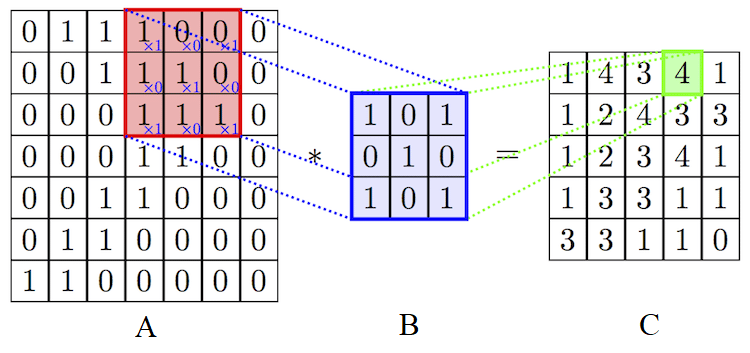
\includegraphics[width=\textwidth]{image/chapter_2/conv-example.png}
		\caption{Пример двумерной свёртки с параметрами: размер ядра~=~3, сдвиг~=~1}
		\label{fig:conv}
	\end{figure}

	В случае фильтра гаусса матрица $B$ равна матрице $G(\sigma)$, элементы которой вычисляются по формуле:
	\begin{equation}
		G(\sigma)_{x,y} = \frac{1}{2\pi\sigma^2}e^{-\frac{(x-m_x/2)^2 + (y-m_y/2)^2}{2\sigma^2}}, 
		\label{eq:G(sigma)}
	\end{equation} 
	где $m_x$ и $m_y$ - размеры свертки.

	Далее находится разности для каждой пары уровней $i$, $j$ по формуле:
	\vspace*{-1.1cm}
	\begin{equation*}
		D\left(x,y,\sigma \right)=L\left(x,y,k_{i}\sigma \right)-L\left(x,y,k_{j}\sigma \right),
		\label{D(x,y,sigma)}
		\vspace*{-0.5cm}
	\end{equation*}
	где $x$, $y$ -- координаты точки $\sigma$ -- параметр размытия, $k_i$ и $k_j$ -- масштаб на некоторых уровнях. На каждом уровне масштаб уменьшается в 2 раза. Это позволяет обнаруживать объекты на разных масштабах;
	
	\item вычисление градиента: Для каждого пикселя на изображении вычисляются значения градиента функции $D$, показывающие направление и величину изменения яркости в этой точке. На основании полученных градиентов определяются локальные экстремумы;
	
	\item удаление низкоконтрастных ключевых точек: Ключевые точки, которые имеют слишком низкий контраст, могут быть удалены, так как они не являются достаточно выраженными;
	
	\item определение масштаба - для каждой особой точки определяется масштаб, используя локальный максимум градиента вокруг точки;
	
	\item определение ориентации - для каждой особой точки определяется направление градиента. Это позволяет сделать дескрипторы инвариантными к повороту изображения. В первую очередь берётся размытое по Гауссу изображение $L\left(x,y,\sigma \right)$ в ключевых точках с масштабом $\sigma$, так что все вычисления осуществляются в масштабно-инвариантной манере. Для изображения $L\left(x,y\right)$ с масштабом $\sigma$  предварительно вычисляются на основе разности пикселей величина градиента 
	$m\left(x,y\right)$ и ориентация $\theta \left(x,y\right)$
	\begin{equation*}
	 	m\left(x,y\right)={\sqrt {\left(L\left(x+1,y\right)-L\left(x-1,y\right)\right)^{2}+\left(L\left(x,y+1\right)-L\left(x,y-1\right)\right)^{2}}};
		\label{m(x,y,sigma)}
		\vspace*{-0.4cm}
	\end{equation*}
	\begin{equation*}
		\hspace{-0.25cm}\theta \left(x,y\right)=\mathrm {atan2} \left(L\left(x,y+1\right)-L\left(x,y-1\right),L\left(x+1,y\right)-L\left(x-1,y\right)\right),
		\label{teta(x,y,sigma)}
			\vspace*{-0.35cm}
	\end{equation*}
	где atan2 -- функция, которая возвращает угол между положительным направлением оси x и лучом, проходящим через начало координат и заданную точку.
	Функция задается следующим образом:
	\begin{equation*}
		\operatorname{atan2}(y, x) = 
		\begin{dcases}
			\arctan\left(\frac{y}{x}\right) + \pi \cdot \frac{1 - \operatorname{sign}(y)}{2} - \pi \cdot \operatorname{sign}(x) \textup{, при } x~\ne~0, \vspace*{0.4cm} \\ 
			\frac{\pi}{2} \textup{, при } x=0 \textup{, } y\ge0, 
			\vspace*{0.4cm} \\ 
			-\frac{\pi}{2} \textup{, при } x=0 \textup{, } y<0, 
		\end{dcases}
		\label{m(x,y,sigma)}
		\vspace*{-0.1cm}
	\end{equation*}
	где $\operatorname{sign}$ -- возвращает знак аргумента. Вычисление величины и направления для градиента делается для каждого пикселя в окрестности ключевой точки в размытом по Гауссу изображении L. Формируется гистограмма направлений с 36 областями, каждая из которых покрывает 10 градусов. Каждая точка в окружающем окне добавляется в область гистограммы, взвешенная по величине градиента и по гауссово-взвешенному круговому окну с $\sigma$, которое в 1,5 раза больше масштаба ключевой точки. Пики в этой гистограмме соответствуют доминирующим направлениям. Как только гистограмма заполнена, направления, соответствующие самым высоким пикам и локальным пикам, которые в пределах 80\% от самых высоких пиков, назначаются ключевой точке. В случае назначения нескольких направлений создаётся дополнительная ключевая точка, имеющая то же местоположение и масштаб, что и оригинальная точка для каждого дополнительного направления;
	\item в первую очередь создаётся набор гистограмм направлений на 4×4 соседних пикселях с 8 областями в каждой. Эти гистограммы вычисляются из значений величины и ориентации элементов в области 16×16 вокруг ключевой точки, так что каждая гистограмма содержит элементы из 4×4 подобласти исходной области соседства. Величины далее взвешиваются функцией Гаусса с $\sigma$, равной половине ширины окна дескриптора. Дескриптор затем становится вектором всех значений этих гистограмм. Поскольку имеется 4~×~4~=~16 гистограмм с 8 областями в каждой, вектор имеет 128 элементов. Этот вектор нормализуется до единичной длины, чтобы обеспечить инвариантность аффинным изменениям в освещении;
	
	\item отбор особых точек - особые точки отбираются на основе надежности дескрипторов, исходя из порогового значения. Кроме того, особые точки могут быть отфильтрованы, если они находятся на границе изображения или находятся в областях с низким контрастом.
	\end{enumerate}

	На этом алгоритм поиска ключевых точек завершается. 
	В результате получаем набор ключевых точек и дескрипторов $A$ для изображения образца и набор точек и дескрипторов $B$ для входного изображения. Далее используем ранее описанный алгоритм <<k ближайших соседей>> для классификации элементов из набора $A$ по $n$ классам, где $n$ -- размер набора $B$. Для этого формируется обучающая выборка, представляющая набор дескрипторов из набора $B$. Далее для каждого элемента $A_i$ получаем некоторый индекс $t_i$, соответствующий номеру класса, получаем вектор сопоставлений $y_i$, вида $[ap_i, ad_i, bp_{t_i}, bd_{t_i}, d_i]$, где $ap_i$ и $ad_i$ -- точка и дескриптор из набора $A$ соответственно, $bp_{t_i}$ и $bd_{t_i}$ -- 
	точка и дескриптор из набора $B$ соответственно, а $d_i$ -- евклидово расстояние между $ad_i$ и $bd_{t_i}$. После этого отсекаем вектора с расстояниями большими определенного порога.
	Используя получившиеся вектора сопоставлений можно восстановить координаты искомого прямоугольника, содержащего трубу. Пренебрегая возможностью поворота трубы, так как тепловизор не будет двигаться с того места куда его установили, сделать это можно имея всего 2 точки, однако возникает проблема выбросов, когда по какой-то причине точки сопоставляются неправильно. Следовательно, необходимо реализовать алгоритм, который будет уметь обрабатывать выбросы и находить наиболее точное соответствие.
	
	Этим требованиям удовлетворяет алгоритм <<RanSaC>>(Random Sample Consensus) -- это итеративный алгоритм для решения задачи нахождения модели в данных, которые содержат выбросы [\ref{FischlerBollesRandomsampleconsensusaparadigmformodelfitting}]. Основная идея алгоритма <<RanSaC>> заключается в том, чтобы выбрать случайным образом некоторое количество точек из исходных данных, и использовать их для построения модели. Затем для каждой точки в данных проверяется, удовлетворяет ли она модели. 
	
	Алгоритм получает на вход координаты границ изображения образца $[x^{a}_{1}, x^{a}_{2}]$ и $[y^{a}_{1}, y^{a}_{2}]$, а также множество векторов сопоставлений, его можно разделить не несколько шагов:
	\begin{enumerate}[label={\arabic*)}]
		\item случайным образом выбираем 2 вектора $y_i$, $y_j$;
		\item вычисляем границы внутренних прямоугольников для входного изображения и изображения образца, для этого находим минимумы и максимумы по координатам $x$ и $y$ точек $ap_i$ и $ap_j$ , и точек $bp_{t_i}$ и $bp_{t_j}$ по следующим формулам:
		\begin{subequations}
		\vspace*{-0.4cm}
			\begin{equation*}
				x_{min} = min(x_{i},~x_{j}),~~~~x_{max} = max(x_{i},~x_{j}),
			\end{equation*}
		\vspace*{-1.4cm}
			\begin{equation*}
				y_{min} = min(y_{i},~y_{j}),~~~~y_{max} = max(y_{i},~y_{j});
			\end{equation*}
		\label{x,y,min,max}
		\end{subequations}
		\item вычислим координаты прямоугольника на изображении образце следующим образом:
		\begin{subequations}
			\begin{equation*}
				x^{b}_{1} = x^{b}_{min} - \frac{(x^{a}_{min} - x^{a}_{1})(x^{b}_{max} - x^{b}_{min})}{x^{a}_{max} - x^{a}_{min}},
			\end{equation*}
			\vspace*{-0.8cm}
			\begin{equation*}
				x^{b}_{2} = x^{b}_{max} + \frac{(x^{a}_{2} - x^{a}_{max})(x^{b}_{max} - x^{b}_{min})}{x^{a}_{max} - x^{a}_{min}},
			\end{equation*}
			\vspace*{-1.1cm}
			\begin{equation*}
				y^{b}_{1} = y^{b}_{min} - \frac{(y^{a}_{min} - y^{a}_{1})(y^{b}_{max} - y^{b}_{min})}{y^{a}_{max} - y^{a}_{min}},
			\end{equation*}
			\vspace*{-1.1cm}
			\begin{equation*}
				y^{b}_{2} = y^{b}_{max} + \frac{(y^{a}_{2} - y^{a}_{max})(y^{b}_{max} - y^{b}_{min})}{y^{a}_{max} - y^{a}_{min}};
			\end{equation*}
			\label{x,y,1,2}
			\vspace*{-0.8cm}
		\end{subequations}
		\item теперь, имея координаты прямоугольника можно вычислить проекции всех точек в модели и рассчитаем сумму расстояний до их реальных положений по формуле:
		\begin{equation}
			dist = \sum\limits_{k=1}^n \sqrt{(u_k)^2 + (v_k)^2},
			\label{dist}
		\end{equation}
		где $n$ -- количество векторов сопоставления, 
		\begin{equation*}
			u_k = x^{b}_{1} + \frac{(x^{a}_{k} - x^{a}_{1})(x^{b}_{max} - x^{b}_{min})}{x^{a}_{max} - x^{a}_{min}} - x^{b}_{k},
			\label{dist1dop}
		\end{equation*}
		\vspace*{-0.8cm}
		\begin{equation*}
			v_k = y^{b}_{1} + \frac{(y^{a}_{k} - y^{a}_{1})(y^{b}_{max} - y^{b}_{min})}{y^{a}_{max} - y^{a}_{min}} - y^{b}_{k};
			\label{dist2dop}
		\end{equation*}
		\item Если $dist$ меньше текущего наилучшего результата, обновим результат;
		\item Увеличиваем счетчик итераций, если счетчик не превысил заданного изначального возвращаемся к п первому шагу.
	\end{enumerate}

	После этого получаем границы прямоугольника, содержащего трубу.

\subsection{Метод сегментации водоразделом (WaterShed)}
	
	Итоговым шагом является непосредственно сегментация факела выбросов. Напомним, что в виду того, что факел выбросов обладает высокой температурой, матрица температуры обладает большей информацией для сегментации.
	
	Для сегментации было решено использовать классические алгоритмы сегментации. Ввиду малого контраста изображения было решено использовать алгоритм <<WaterShed>> или метод сегментации водоразделом, так как этот алгоритм наилучшим образом работает с низко-контрастными изображениями.
	
	Рассмотрим некоторые математические понятия, необходимые нам для описания математической модели алгоритми сегментации водоразделами. Рассмотрим понятие секции уровня $Z_i(f)$ как следующее множество:
	\begin{equation*}
		Z_i(f) = \{x\in \mathbb{Z}^2:~f(x)\le i\}.
		\label{Z_i(f)}
	\end{equation*}
	
	Рассмотрим математическую модель данного алгоритма. Для этого введем понятие геодезического расстояния $d_X(x,y)$ между некоторыми точками $x$ и $y$, принадлежащими некоторому множеству $X$. Данное расстояние будем считать равным длинне кратчайшего пути, соединяющего $x$ и $y$ и принадлежащего множеству $X$ (если таковой существует). Путем $p(x,y)$ будем называть некоторую последовательность точек $s$, состоящую из $n$ точек, для которой справедливо, что $s_i$ и $s_{i+1}$ яляются соседними точками, для $\forall i~\in~[0,~n-1]$, где $s_0 = x$ и $s_n = y$. Длинна такого пути будет равна $n$ (см.~рисунок~\ref{fig:gerodesic_distance}).
	
	\begin{figure}[h!]
		\centering
		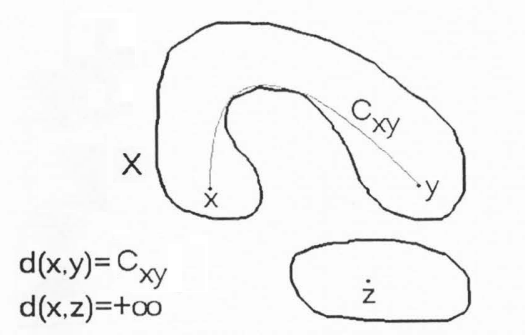
\includegraphics[width = 0.5\textwidth]{image/chapter_2/gerodesic_distance}	
		\caption{Пример геодезического \\ расстояния}
		\label{fig:gerodesic_distance}
	\end{figure}
	Также введем понятие топографической поверхности как множества точек вида $\{x, f(x)\}$. Тогда не восходящий путь между двумя точками $s_1(x_1,f(x_1))$ и $s_2(x_2,f(x_2))$ определим как некоторый путь, такой, что все точки включенные в путь отвечают следующему условию:
	\begin{equation*}
		\forall s_i(x_i,~f(x_i)),~s_j(x_j,~f(x_j)):~i\ge j \Leftrightarrow f(x_i) \le f(x_j).
		\label{z_X(Y_i)}
	\end{equation*}
	Тогда локальным минимумом назовем точку, из которой не существует не восходящих путей, локальным максимумом назовем точку, все пути из которой являются невосходящими (см.~рисунок~\ref{fig:loc_watershed}). Распределим локальные минимумы в некоторый набор множеств $M_k$, таких, что:
	\begin{equation*}
		\forall s_i(x_i,~f(x_i)),~s_j(x_j,~f(x_j)) \in M_k:~\exists p(s_i,~s_j) \in M_k.
		\label{z_X(Y_i)}
	\end{equation*}
	 
	\begin{figure}[h!]
		\begin{subfigure}{.45\textwidth}
			\centering
			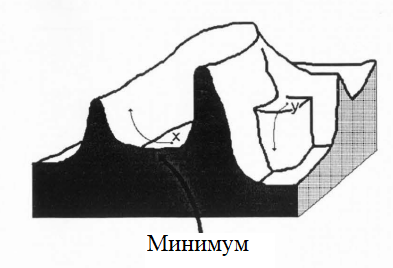
\includegraphics[width = \textwidth]{image/chapter_3/loc_min_watershed}
			\caption{}
		\end{subfigure}
		\begin{subfigure}{.45\textwidth}
			\centering
			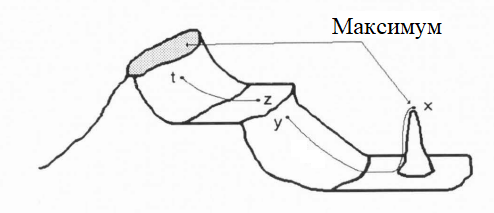
\includegraphics[width = \textwidth]{image/chapter_3/loc_max_watershed}
			\caption{}
		\end{subfigure}
		\centering
		\caption{Пример локальных: a) минимума; б) максимума}
		\label{fig:loc_watershed}
	\end{figure}
	
	Други важным понятием является геодезическая зона влияния. Пусть cуществует последовательность непересекающихся подмножеств $Y_i\in X$. Тогда геодезическую зону влияния подмножества $Y_i$ определим следующим образом:
	 \begin{equation*}
	 	\textup{z}_X(Y_i) = \{x\in X:d_X(x,Y_i)\textup{ конечна, }\forall j\ne i,~d_X(x,Y_j)>d_X(x,Y_i)\}.
	 	\label{z_X(Y_i)}
	 \end{equation*}
 
 	Определим также границы зон влияния $\textup{SKIZ}_X(Y)$ (см.~рисунок~\ref{fig:SKIZ}) следующим образом:
 	 \begin{equation*}
 		\textup{SKIZ}_X(Y) = X~/~\textup{IZ}_X(Y),
 		\label{SKIZ_X(Y)}
 	\end{equation*}
	где:
	\begin{equation*}
		\textup{IZ}_X(Y) = \bigcup_{i} \textup{z}_X(Y_i).
		\label{IZ_X(Y)}
	\end{equation*}

	\begin{figure}[h!]
		\centering
		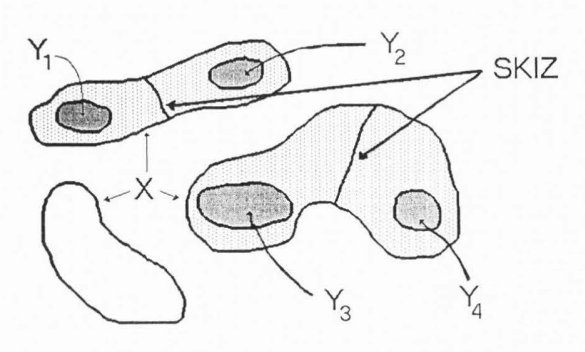
\includegraphics[width = 0.6\textwidth]{image/chapter_2/SKIZ}	
		\caption{Пример нахождения зон \\влияния и их границ}
		\label{fig:SKIZ}
	\end{figure}
	
	Теперь представим изображение в виде топографической поверхности. Предположим теперь что мы делаем проколы во всех связных множествах $M_i$ и погружаем топографическую поверхность с постоянной скоростью под воду. Во время наводнения два или более потоков воды (из разных $M_i$) могут соеденится воедино, чтобы это предотвратить мы строим плотины в тех местах где они сталкиваются. После этого остаются только плотины, компоненты связности образованные этими плотинами назовем басейнами и обозначим $\textup{CB}_i$, каждая из которых представляет ровно одному связному множеству $M_i$. Пример затопления представлен на рисунке~\ref{fig:potop_watershed}.
	\begin{figure}[h!]
		\begin{subfigure}{.49\textwidth}
			\centering
			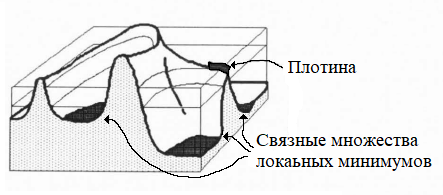
\includegraphics[width = \textwidth]{image/chapter_3/potop1_watershed}
			\caption{}
		\end{subfigure}
		\begin{subfigure}{.49\textwidth}
			\centering
			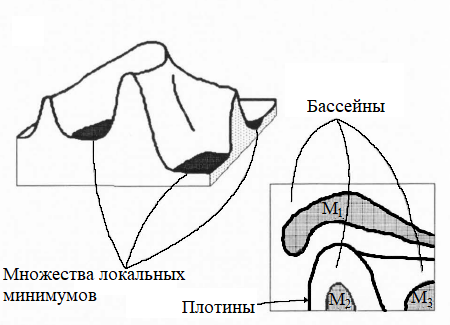
\includegraphics[width = \textwidth]{image/chapter_3/potop2_watershed}
			\caption{}
		\end{subfigure}
		\centering
		\caption{Пример затопления: a) последовательные уровни затопления; б) сопоставление поверхности с видом сверху}
		\label{fig:potop_watershed}
	\end{figure}

	Более строгое математическое описание данного алгоритма можно привести используя ранее введенные нами термины.
	

\chapter[\vspace*{-0.22cm}РАЗРАБОТКА И ПРОГРАММНАЯ РЕАЛИЗАЦИЯ АЛГОРИТМА \hspace*{-0.5cm} СЕГМЕНТАЦИИ ФАКЕЛА ВЫБРОСОВ]{\vspace*{-0.22cm}РАЗРАБОТКА И ПРОГРАММНАЯ РЕАЛИЗАЦИЯ АЛГОРИТМА СЕГМЕНТАЦИИ ФАКЕЛА ВЫБРОСОВ}
\section[Разработка алгоритма подготовки данных]{Разработка алгоритма подготовки данных}

	Первым этапом подготовки данных является получение этих данных с тепловидео систем наблюдения. Для этого нужно разработать алгоритм взаимодействия с тепловизором и научиться получать данные для последующей обработки. Как уже было описано выше разработчики теплоаизора предоставляют пакет SDK, а также библиотеку для работы с тепловизором.
	Для решения нашей задачи необходимо обеспечить синхронную запись оптических снимков и тепловых карт, соответствующих этим снимкам. Несмотря на то, что SDK предоставляет возможность получения полной матрицы температур, этот способ был признан неэффективным, так как библиотека позволяет выполнять подобный запрос с периодичностью раз в секунду. Было решено записывать незакодированные оптические и тепловые снимки в формате YUV (см. рисунки~\ref{fig:opt_example},~\ref{fig:tep_example}). 
	\begin{figure}[h!]
		\centering
		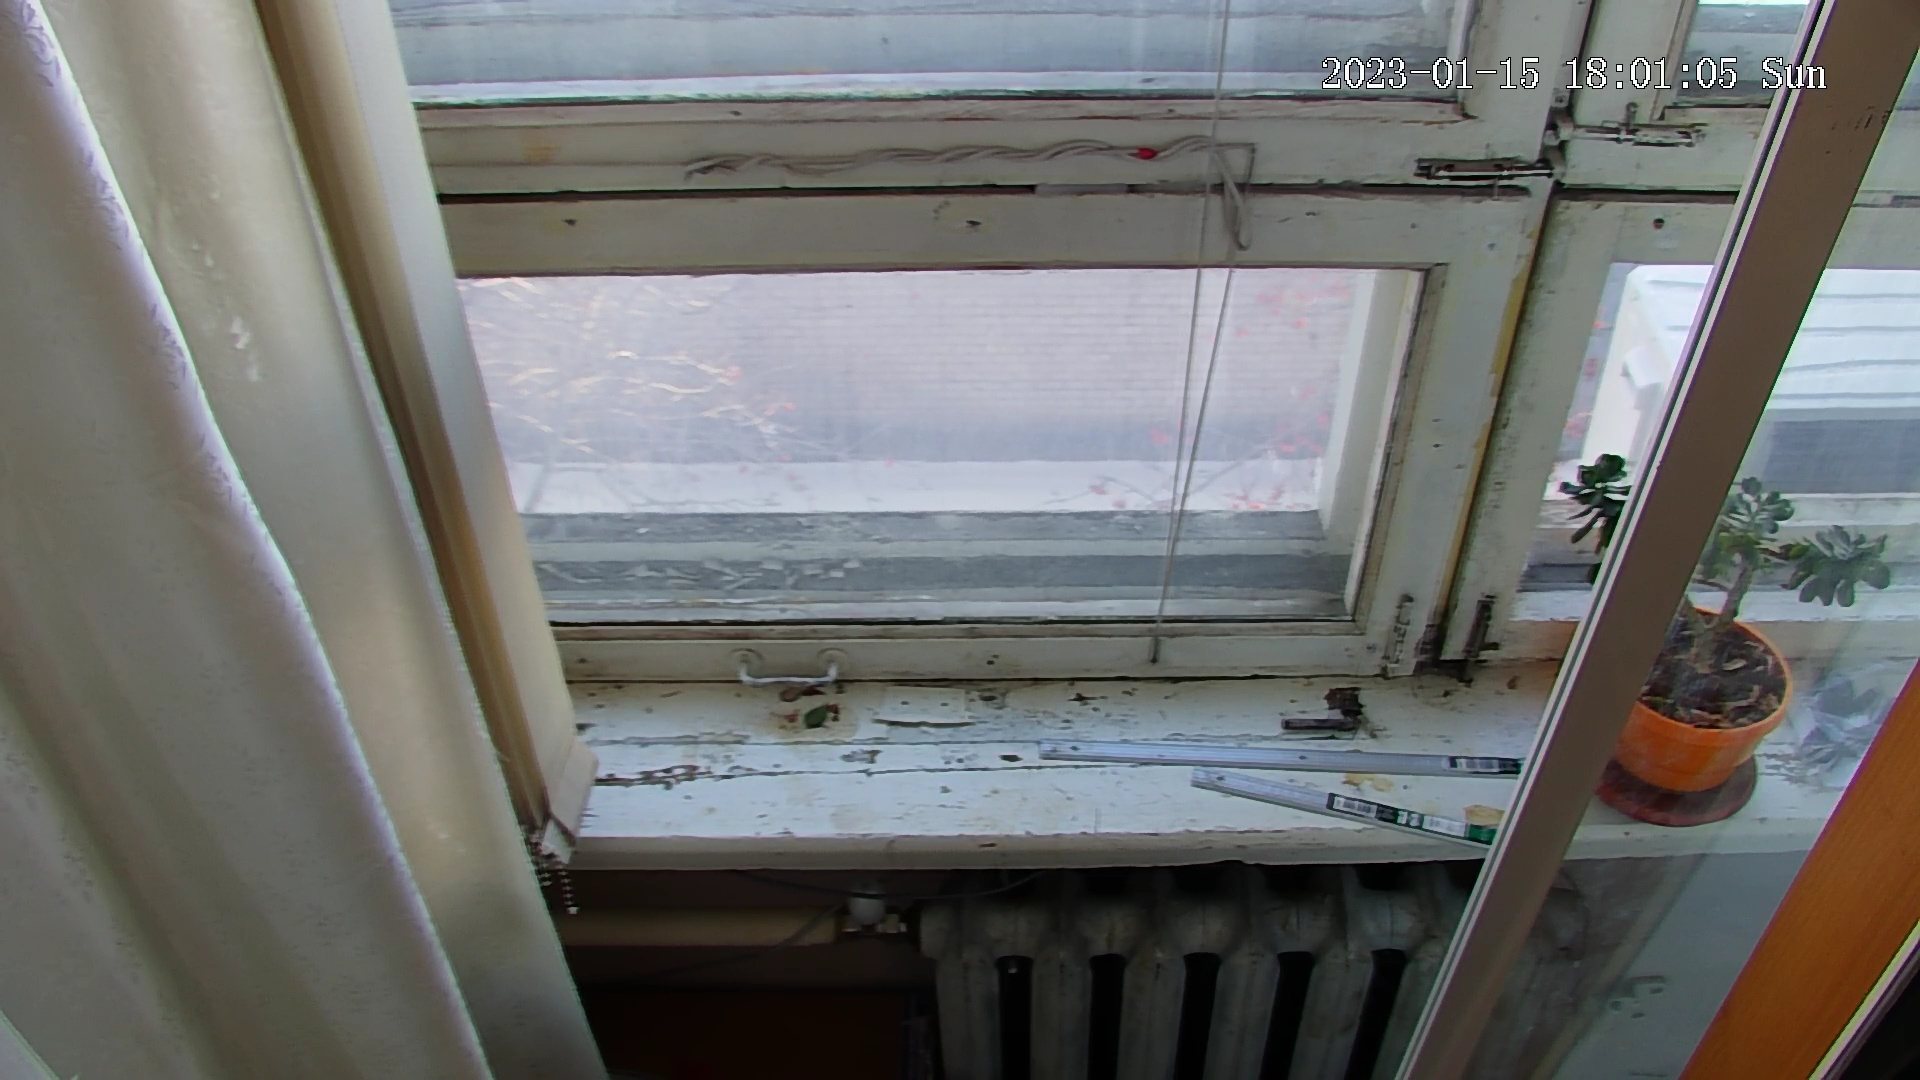
\includegraphics[width = 13cm]{image/chapter_2/opt_example}	
		\caption{Пример оптического снимка}
		\label{fig:opt_example}
	\end{figure}
	
	\begin{figure}[h!]
		\centering
		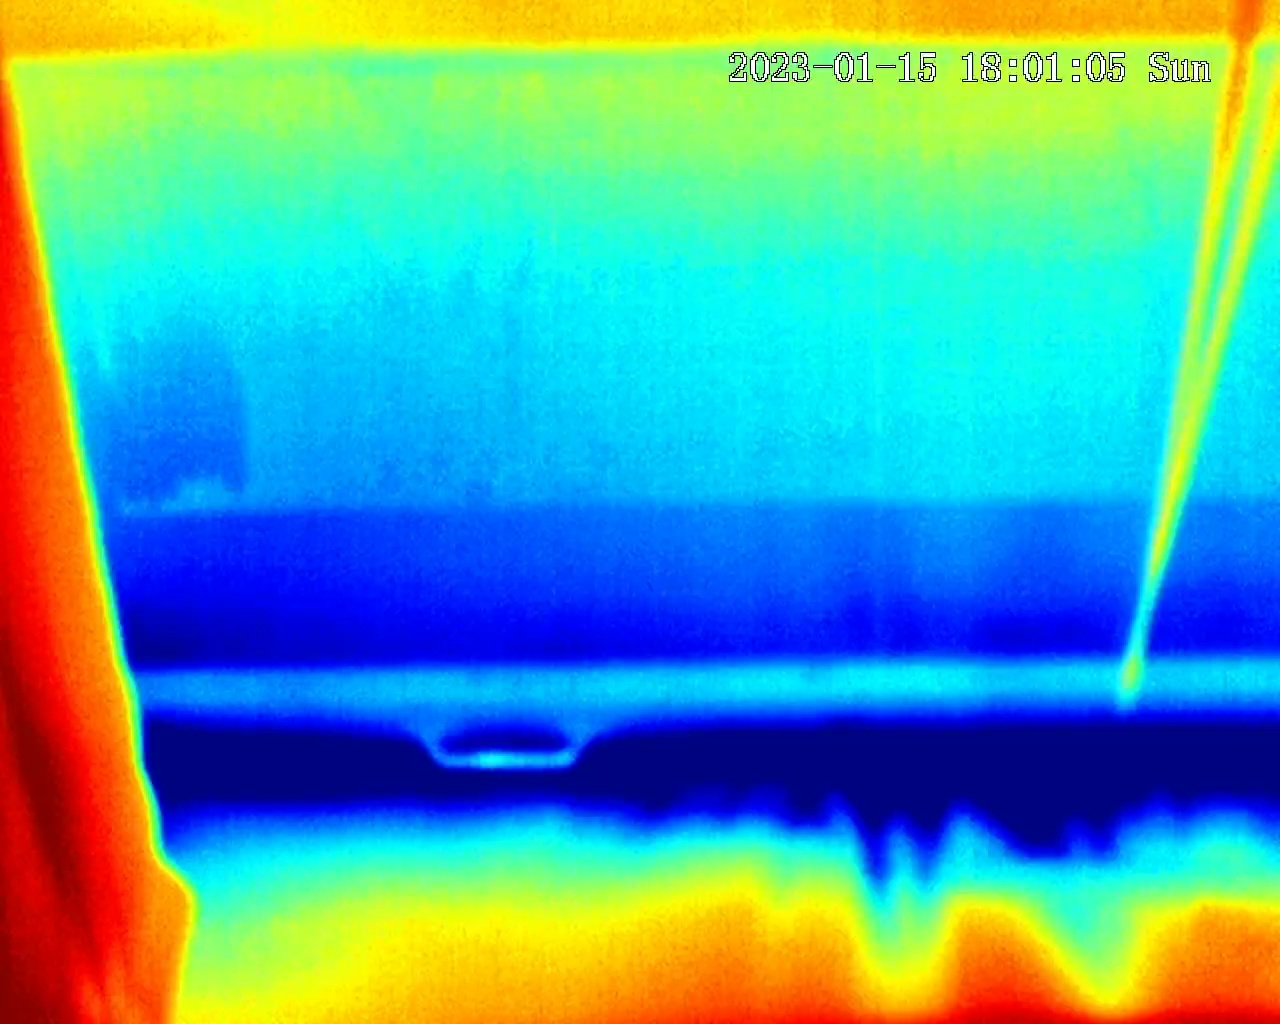
\includegraphics[width = 0.6\textwidth]{image/chapter_2/tep_example}	
		\caption{Пример теплового снимка}
		\label{fig:tep_example}
	\end{figure}
	Для обеспечения синхронности и стабильности было решено снизить частоту кадров с 25 Гц до 20 Гц. Также с частотой в 1 Гц производится считывание полной матрицы температур для определения максимальной и минимальной температуры. 
	
	В результате был разработан алгоритм записи оптических и тепловых снимков. Схема алгоритма записи представленна на рисунке~\ref{fig:loaddata}.
	
	\begin{figure}[h!]
		\centering
		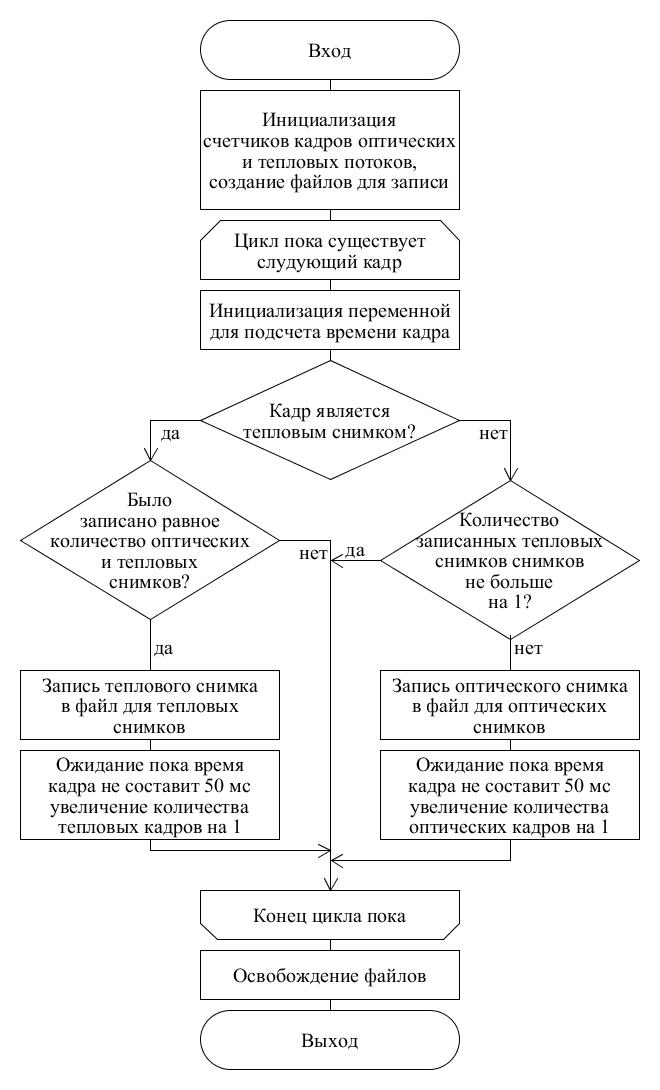
\includegraphics[width = 0.7\textwidth]{image/chapter_2/loaddata}	
		\caption{Схема алгоритма записи\\ оптических и тепловых снимков}
		\label{fig:loaddata}
	\end{figure}
	
	Следующим этапом подготовки данных является ранее описанное преобразование цветовой карты. Необходимо преобразовать изоражение из формата цветовой карты <<JET>> к оттенкам серого, иными словами разработать алгоритм, востанавливающий целевую функцию~(\ref{eq:gYX}), удовлетворяющий поставленным ранее требованиям.
	
	Для этого в соответствии с ранее описанной математической моделью необходимо подготовить алгоритм классификатора цветов, заключающийся в составлении обучающей выборки и обучении на ней ранее рассмотреной модели <<flannBasedMatcher>> и после классификации пикселей из пространства RGB. Математическая модель была описана ранее.  
	
	В результате был разработан алгоритм преобразования изображения в цветовой карте <<JET>> в изображение в оотенках серого. Итоговый алгоритм преобразования имеет вид (см.~рисунок~\ref{fig:colorclassification}).
	
	\begin{figure}[h!]
		\begin{subfigure}{.6\textwidth}
			\centering
			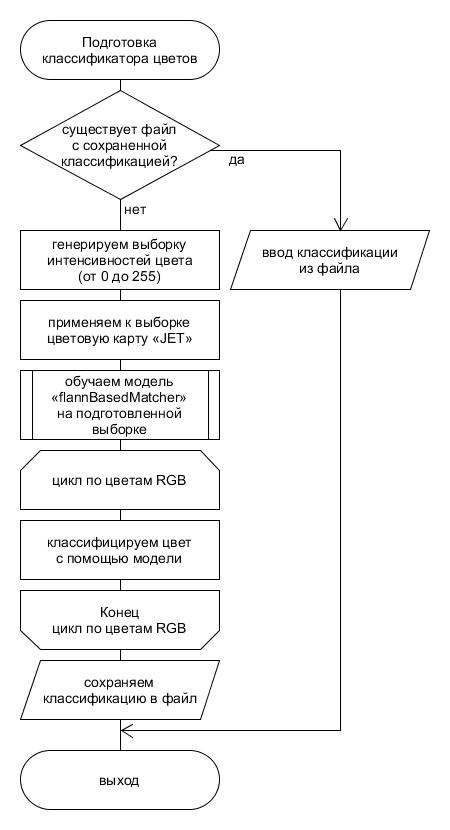
\includegraphics[width = \textwidth]{image/chapter_2/colorclassification}
			\caption{}
		\end{subfigure}
		\begin{subfigure}{.31\textwidth}
			\centering
			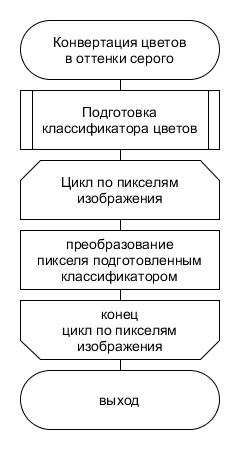
\includegraphics[width = \textwidth]{image/chapter_2/colorclassification2}
			\caption{}
		\end{subfigure}
		\centering
		\caption{Схема алгоритмов преобразования цветовой карты: \\a) преобразование пространства RGB; б) преобразование изображения}
		\label{fig:colorclassification}
	\end{figure}
	Примером работы данного алгоритма является римунок~\ref{fig:grey1}.
	\begin{figure}[h!]
		\centering
		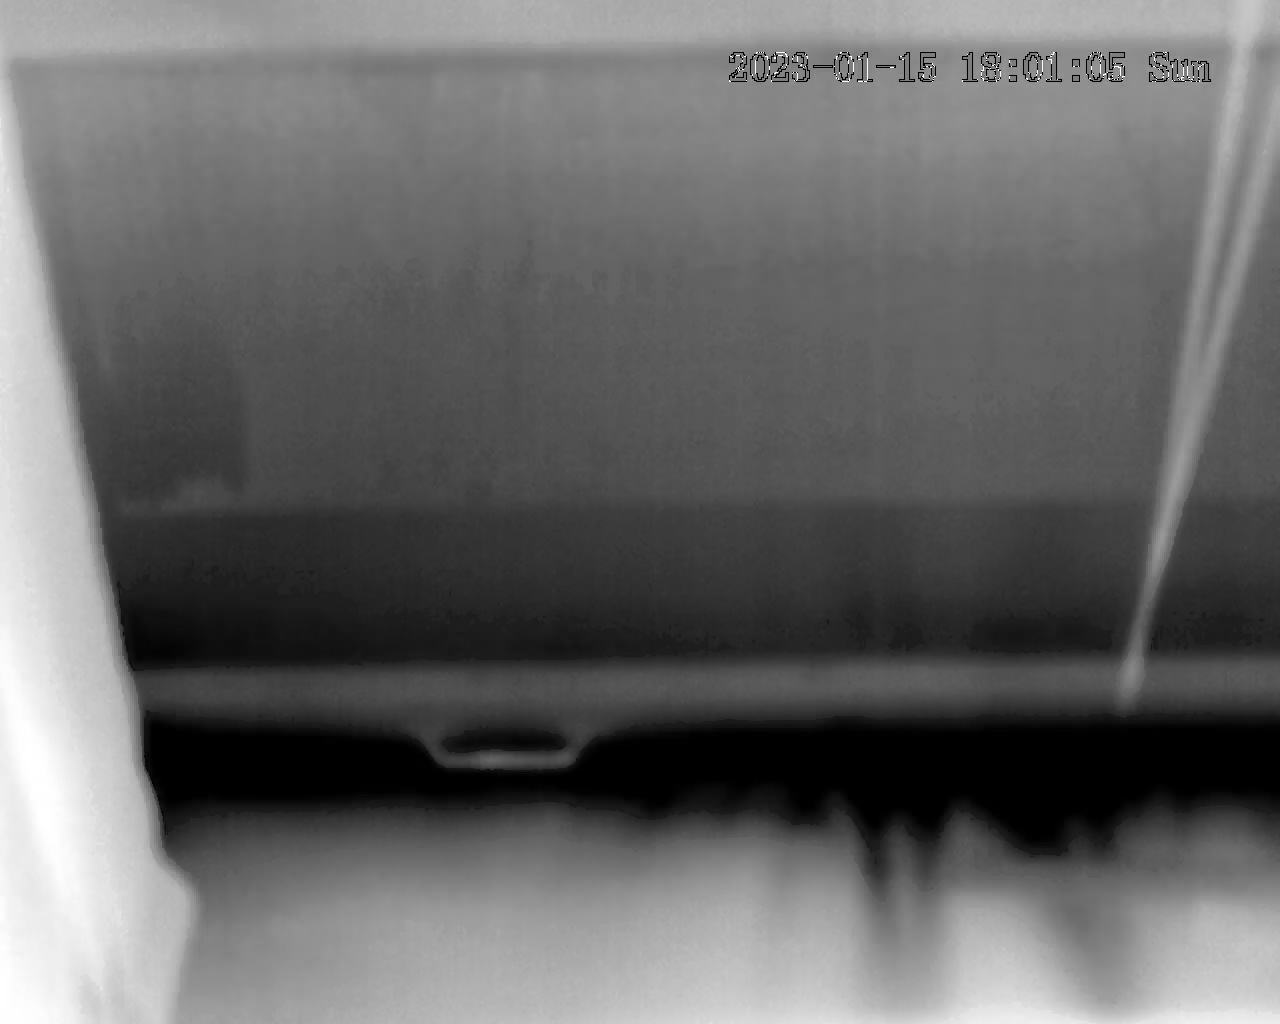
\includegraphics[width = 0.9\textwidth, height = 0.475\textwidth]{image/chapter_2/gray_tep_example}
		\vspace*{-0.2cm}	
		\caption{Результат работы алгоритма преобразования цветов}
		\label{fig:grey1}
		\vspace*{0.4cm}
	\end{figure}
	Рассмотрим точность работы получившигося алгоритма. Для оценки точности функции была сформирована тестовая выборка представляющая собой изображение $P^{true}$ (см.~рисунок~\ref{fig:grey1}) в оттенках серого и изображение $P^{conv}$ (см.~рисунок~\ref{fig:grey2}) преобразованное к цветовой карте <<JET>> и сжатое с помощью технологии сжатия JPEG, а после преобразованная с помощью оцениваемой модели. Введена следующая метрика точности:
	\begin{equation}
		Acc = 1 - \frac{\sum\limits_{i=1}^h \sum\limits_{j=1}^w |P^{true}_{ij} - P^{conv}_{ij}|}{255wh},
		\label{eq:flanaccuracy}
	\end{equation}
	\begin{figure}[h!]
		\centering
		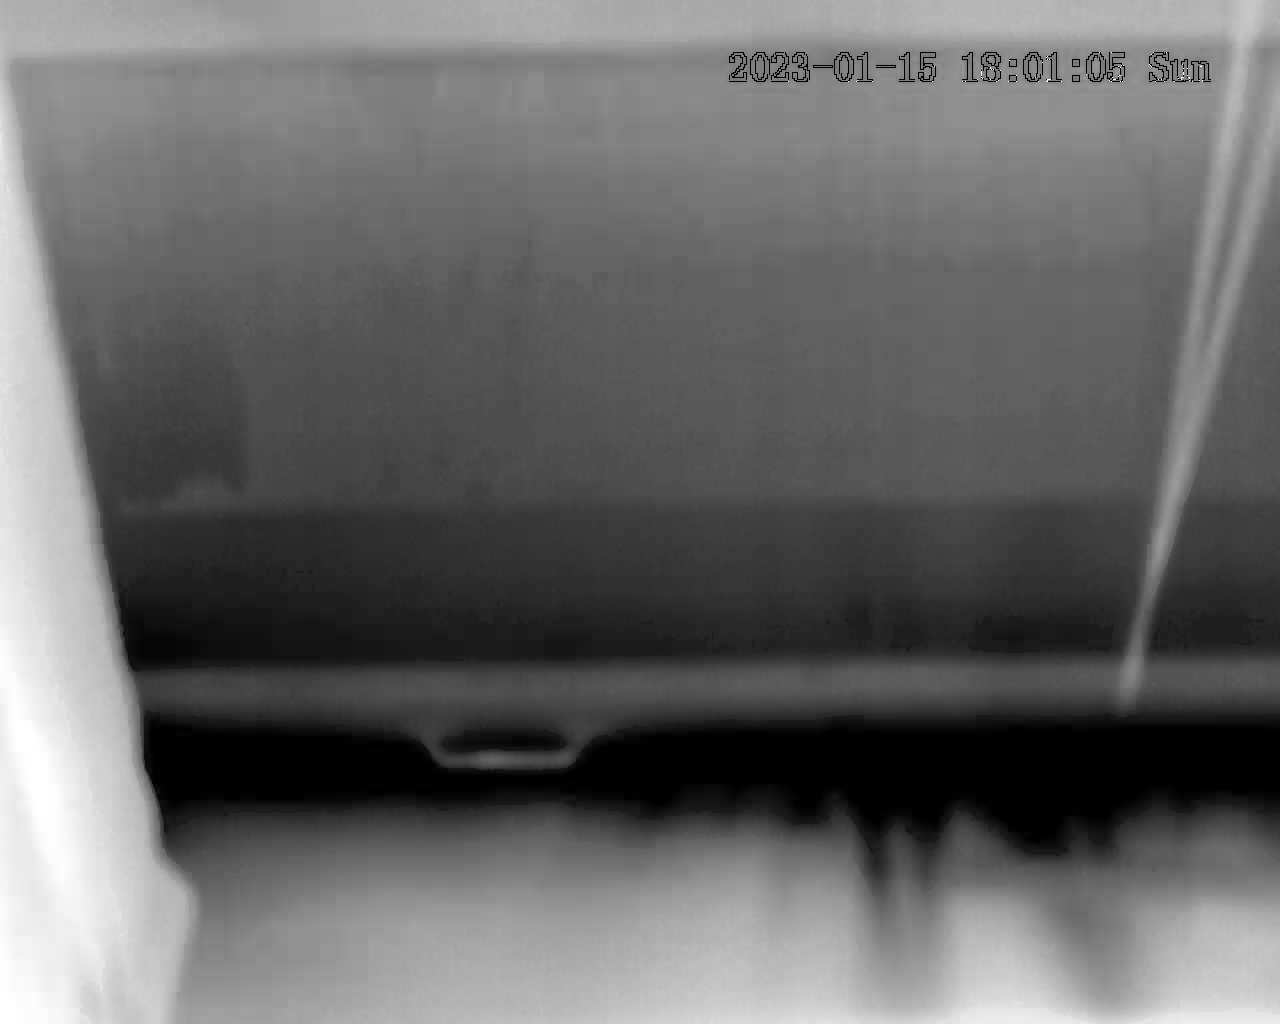
\includegraphics[width = 0.9\textwidth, height = 0.475\textwidth]{image/chapter_2/grey2}
		\vspace*{-0.2cm}
		\caption{Сжатое изображение после применения модели}
		\label{fig:grey2}
	\end{figure}
	где $w$ и $h$ -- высота и ширина изображений $P^{true}$ и $P^{conv}$ соответственно. В результате была получена точность 0,995777. Такая точность позволяет \\ говорить, что примененная модель достаточно точно востанавливает целевую функцию~(\ref{eq:gYX}).
	
	Следующим этапом является наложение преобразование относительных температур к абсолютным. Для этого преобразовываем температуры по формуле~\ref{eq:T_abs}. Далее произведем сдвиг по формуле~\ref{fig:nalozhenie}.
	\begin{figure}[h!]
		\centering
		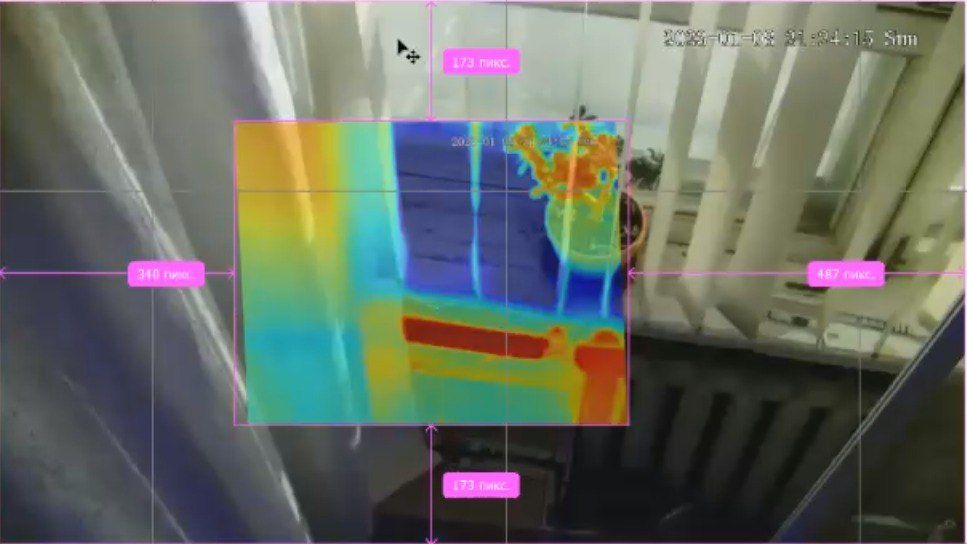
\includegraphics[width = 13cm]{image/chapter_2/nalozhenie}	
		\caption{Пример работы наложения оптического и\\теплового снимков}
		\label{fig:nalozhenie}
	\end{figure}
	
	В результате проделанной работы был разработан алгоритм подготовки данных для решения поставленных задач. Данный алгоритм реализует все 3 этапа подготовки данных с достаточной точностью для любой степени сжатия. При этом благодаря используемым можелям машинного обучения время, затрачиваемое на подготовку данных удалось существенно сократить. Разработанный алгоритм представлен в виде блок схемы, которую можно увидеть на рисунке~\ref{fig:fullprepare}.
	\vspace*{-0.2cm}
	\begin{figure}[h!]
		\centering
		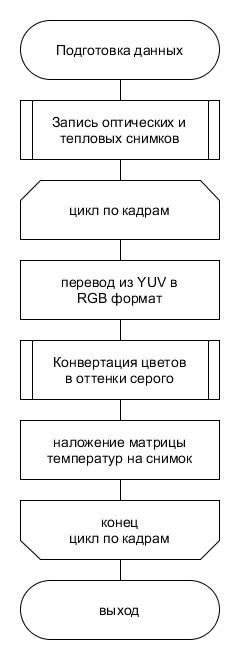
\includegraphics[width = 0.3\textwidth]{image/chapter_2/fullprepare}	
		\vspace*{-0.4cm}\caption{Схема алгоритма \\подготовки кадров}
		\label{fig:fullprepare}
	\end{figure}
	\newpage

\section[\vspace*{-0.22cm}Алгоритм сегментации факела выбросов с помощью оптических \\ \hspace*{-0.75cm}и тепловых снимков]{\vspace*{-0.22cm}Алгоритм  факела выбросов с помощью оптических и тепловых \\ \hspace*{-2.05cm}снимков}
\subsection{Алгоритм детекции трубы}
	
	Для сегментации трубы необходимо решить еще одну важную подзадачу, а именно -- детекцию источника выбросов. Важность этого шага, постановка задачи и математическая модель были описаны ранее, сейчас рассмотрим непосредственно алгоритм детецкии трубы и результаты его работы.
	
	В алгоритме детекции трубы можно выделить несколько важных подзадач. Одна из таких задач -- поиск ключевых точек. Алгоритм поиска ключевых точек показан на рисунке~\ref{fig:trubadetection}.
	\begin{figure}[h!]
		\centering
		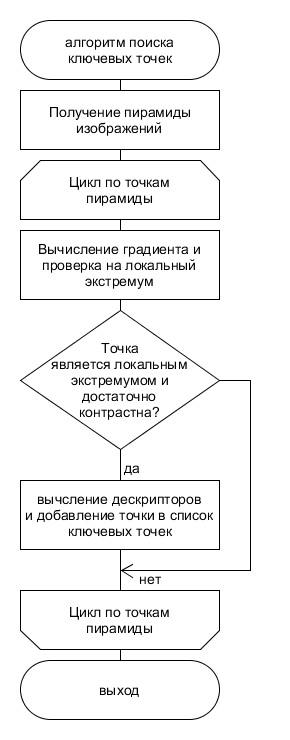
\includegraphics[width = 0.4\textwidth]{image/chapter_3/trubadetection}	
		\vspace*{-0.4cm}\caption{Схема алгоритма \\поиска ключевых точек}
		\label{fig:trubadetection}
	\end{figure}

	Данный алгоритм успешно находит ключевые точки на изображении. Пример работы алгоритма представлен на рисунке~\ref{fig:keypoints}.
	\begin{figure}[h!]
		\centering
		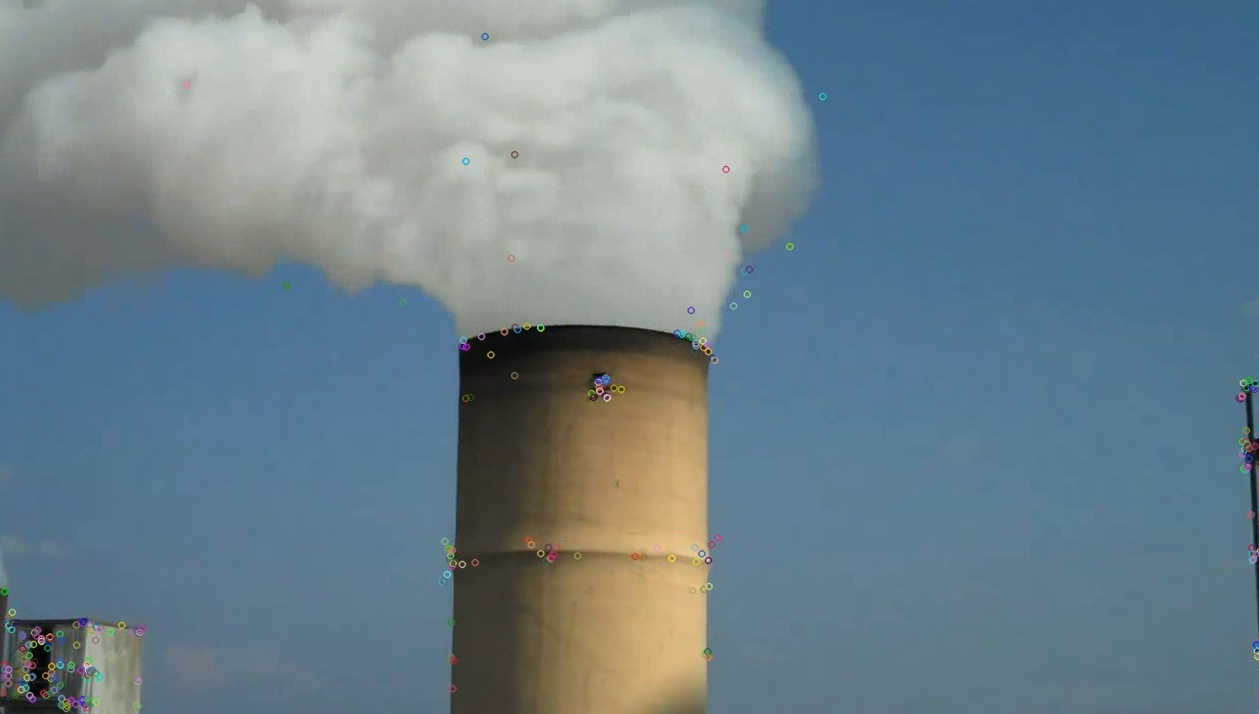
\includegraphics[width = 0.7\textwidth]{image/chapter_2/keypoints}	
		\caption{Пример нахождения ключевых точек}
		\label{fig:keypoints}
	\end{figure}
	
	Следубщим шагом является сопоставление ключевых точек образца и изображения на котором необходимо детектировать трубу. В результате получаем набор ключевых точек и дескрипторов $A$ для изображения образца и набор точек и дескрипторов $B$ для входного изображения. Далее используем ранее описаный алгоритм <<k ближайших соседей>> для классификации элементов из набора $A$ по $n$ классам, где $n$ -- размер набора $B$. Согласно ранее рассмотренной происходит обучение и классификация. Пример работы алгоритма показан на рисунке~\ref{fig:match1}.
	\begin{figure}[h!]
		\centering
		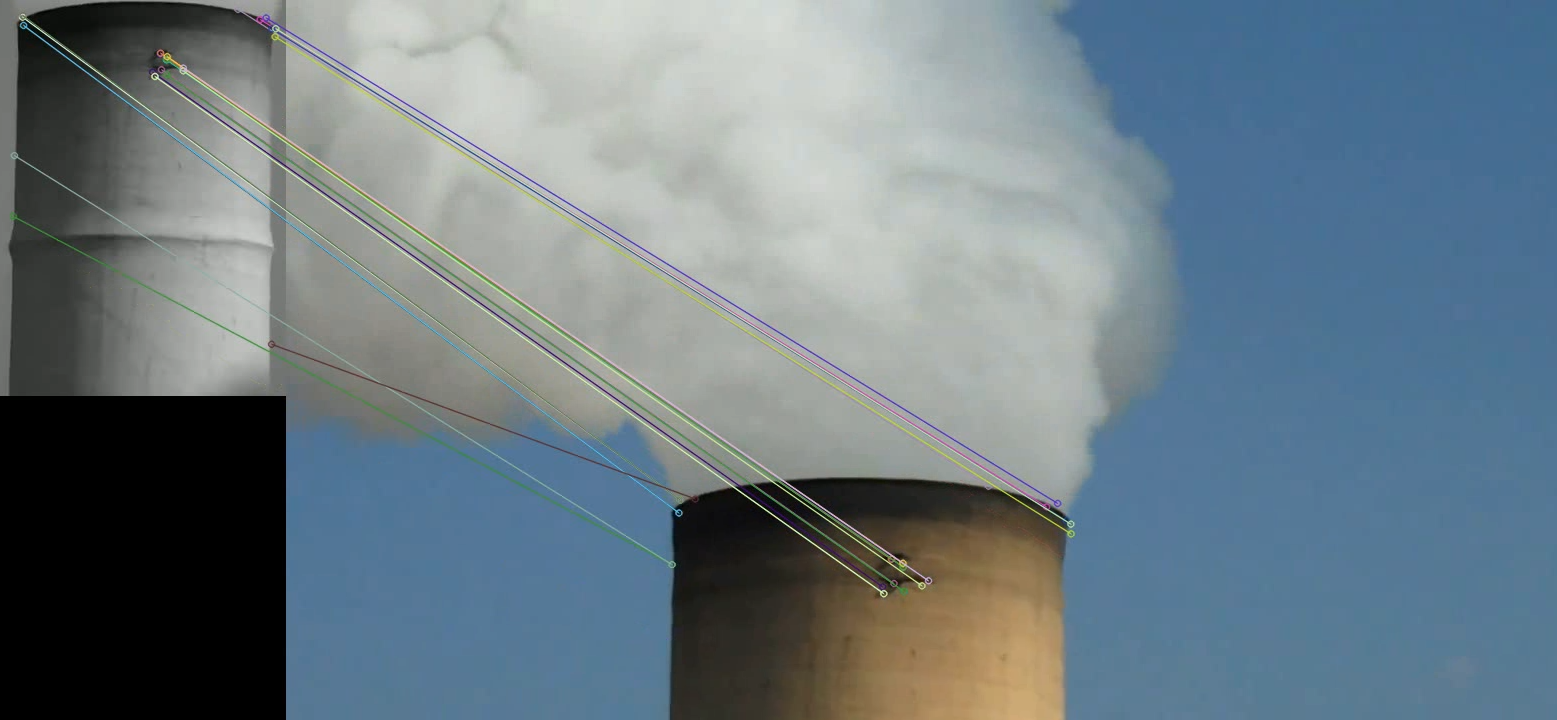
\includegraphics[width = 0.8\textwidth]{image/chapter_2/match1}	
		\caption{Пример сопоставления ключевых точек}
		\label{fig:match1}
	\end{figure}

\chapter*{БИБЛИОГРАФИЧЕСКИЙ СПИСОК}
\addcontentsline{toc}{chapter}{БИБЛИОГРАФИЧЕСКИЙ СПИСОК}

	\begin{sortedlist_rus}
		\sortitem{Группа компаний <<Лаборатория>>: Контроль выбросов в атмосферу: [сайт]. -- 2012. URL: https://gklab.ru/uslugi/proizvodstvennyj-kontrol/\linebreak kontrol-vybrosov-v-atmosferu/ (дата обращения: 10.12.2022).}{gklab.ru}{adarauaqaqaaalapanaqaaaoajakamaaabaparaaataparajbgalapaoatarapambbacbcabarapasapacacaaatanapasavafarau}
		\sortitem{\textbf{Исаев, Л.Н.} Газоанализаторы для контроля атмосферного воздуха и промышленных выбросов / Л.Н.~Исаев, В.Г.~Челибанов // Электронника: ЭТБ: Сетевой журнал. -- 2008. -- №~1. -- C.~34. -- URL:~https://\linebreak www.electronics.ru/files/article\_pdf/0/article\_321\_86.pdf (дата обращения: 10.12.2022).}{electronics.ru}{ajasaaafacayafamajabaaaoapac}
		\sortitem{Газоанализаторы: Классификация газоанализаторов: [сайт]. -- 2017. URL: https://gazoanalizators.ru/articles/klassifikatsiya-gazoanalizatorov/ (дата обращения: 13.12.2022).}{gazoanalizators.ru1}{adaaaiapaaaoaaamajaiaaataparbcalamaaasasajavajalaaaxajbgadaaaiapaaaoaaamajaiaaataparapac}
		\sortitem{Газоанализаторы: Контроль технологических процессов: системы экологического мониторинга промышленных выбросов: [сайт]. -- 2017.\linebreak  URL: https://gazoanalizators.ru/articles/sistemy-ekologicheskogo-monitoringa-promyshlennykh-vybrosov/ (дата обращения: 13.12.2022).}{gazoanalizators.ru2}{adaaaiapaaaoaaamajaiaaataparbcalapaoatarapambbatafawaoapamapadajayafasalajawaqarapaxafasasapacasajasatafanbcbealapamapadajayafasalapadapanapaoajataparajaoadaaaqarapanbcazamafaoaobcawacbcabarapasapac}
		\sortitem{\textbf{Методическое пособие по аналитическому контролю выбросов загрязняющих веществ в атмосферу} /  В.В.~Цибульский,\linebreak Л.И.~Короленко, М.А.~Яценко-Хмелевская, О.Р.~Синицына, М.В.~Боровкова. -- Санкт-Петербург: ОАО <<НИИ АТМОСФЕРА>>, 2012. -- 25~c.}{МЕТОДИЧЕСКОЕ ПОСОБИЕ ПО АНАЛИТИЧЕСКОМУ КОНТРОЛЮ ВЫБРОСОВ ЗАГРЯЗНЯЮЩИХ ВЕЩЕСТВ В АТМОСФЕРУ}{axajabauambbasalajakalaparapamafaoalapbgaxafaoalapawanafamafacasalaabgasajaoajaxbcaoaaabaparapacalapacaa}
		\sortitem{\textbf{Об утверждении методов расчетов рассеивания выбросов вредных (загрязняющих) веществ в атмосферном воздухе} [текст]: Приказ министерства природных ресурсов и экологии Российской Федерации от 6 июня 2017 года № 273 // Министерство природных ресурсов и экологии Российской Федерации, 2017. -- 1--10~c.}{Об утверждении методов расчетов рассеивания выбросов вредных (загрязняющих) веществ в атмосферном воздухе}{apabauatacafarahaeafaoajajanafatapaeapacaraaasayafatapacaraaasasafajacaaaoajbgacbcabarapasapacacarafaeaobcawaiaaadarbgaiaobgbfbaajawacafbaafasatacacaaatanapasavafaraoapanacapaiaeauawaf}
		\sortitem{\textbf{Драгун,~В.Л.} Тепловизионные системы в исследовании тепловых процессов / В.Л.~Драгун, С.А.~Филатов. -- Москва: Наука, 1967. -- 256 с.}{Тепловизионные системы в исследовании тепловых процессов}{aearaaadauaoavajamaaatapac}
		\sortitem{\textbf{Криксунов,~Л.З.} Тепловизоры: справочник / Л.З.~Криксунов, Г.А.~Падалко  -- Киев: Техника, 1987. -- 287 с.}{Тепловизоры: справочник}{alarajalasauaoapacaqaaaeaaamalap}
		\sortitem{\textbf{Виндерлих,~М.Е.} Использование Тепловизора в комплексной диагностике и лечении заболеваний опорно-двигательной системы: обзор литературы / М.Е.~Виндерлих, Н.Б.~Щеколова -- Йошкар-Ола: Марийский государственный университет, 2020. -- 55 с.}{Использование Тепловизора в комплексной диагностике и лечении заболеваний опорно-двигательной системы}{acajaoaeafaramajawbaafalapamapacaa}
		\sortitem{Вики-конспекты: К-d деревья и перечисление точек в произвольном прямоугольнике (статика): [сайт]. -- 2022. URL: https:/clck.ru/nRrXB (дата обращения: 18.03.2023).}{k-мерное дерево на сайте итмо}{acajalajalapaoasaqafalatbcalaeaeafarafacbbbgajaqafarafayajasamafaoajafatapayafalacaqarapajaiacapambbaoapanaqarbganapauadapambbaoajalafasataaatajalaa}
		\sortitem{\textbf{Основы тепловидения}: учебное пособие /  В.В.~Коротаев,\linebreak Г.С.~Мельников, С.В.~Михеев, В.М.~Самков, Ю.И.~Солдатов. --\linebreak Санкт-Петербург: Санкт-Петербургский национальный исследовательский университет информационных технологий, механники и оптики, 2012. -- 123~c.}{Основы тепловидения: учебное пособие}{alaparapataaafacanafambbaoajalapacanajawafafacasaaanalapacasapamaeaaatapac}
	\end{sortedlist_rus}
	\begin{sortedlist_eng}
		\sortitem{\textbf{Lee,~J.} FLIR Technology: 'New' Technology Shines a Camera on Greenhouse Gas Emissions / J.~Lee // Triple Pundit. -- 2018. -- №~12 -- P.~1 URL: https://clck.ru/34N7zc (дата обращения: 02.01.2023).}{triplepundit.com}{LeeJFLIRTechnologyNewTechnologyShinesaCameraonGreenhouseGasEmissions}
		\sortitem{\textbf{Davison,~J.} Gasoline and diesel passenger car emissions deterioration using on-road emission measurements and measured mileage / J.~Davison, R.A.~Rose, N.J.~Farren // Atmospheric Environment: X. -- 2022. -- V.~14. -- P.~100162.}{Gasoline and diesel passenger car emissions deterioration using on-road emission measurements and measured mileage}{DavisonRoseFarren}
		\sortitem{OpenCV: Feature Detection and Description: [сайт]. -- 2018. URL: https://docs.opencv.org/4.x/dc/dc3/tutorial\_py\_matcher.html (дата обращения: 01.02.2023).}{OpenCV: Feature Detection and Description}{OpenCVFeatureDetectionandDescription}
		\sortitem{Automation Technology: Early fire detection and condition monitoring: [сайт]. -- 2020. URL: https://www.automationtechnology.de/cms/wp-content/\linebreak uploads/2015/12/Monitoring-application-overview.pdf (дата обращения:\linebreak 08.02.2023).}{Early fire detection and condition monitoring}{Earlyfiredetectionandconditionmonitoring}
		\sortitem{\textbf{Moreland,~K.D.} Diverging Color Maps for Scientific Visualization (Expanded) / K.D.~Moreland // Sandia National Laboratories. -- 2009. -- P.~3.}{Diverging Color Maps for Scientific Visualization (Expanded)}{MorelandKDDivergingColorMapsforScientificVisualizationExpanded}
		\sortitem{\textbf{Ibraheem,~N.A.} Understanding color models: a review /\linebreak N.A.~Ibraheem, M.M.~Hasan, R.Z.~Khan // Journal of science and technology. -- 2009. -- V.~2, №~3. -- P.~265--275.}{Understanding color models: a review}{Understandingcolormodelsareview}
		\sortitem{\textbf{Cunningham,~P.} k-Nearest neighbour classifiers: a tutorial /\linebreak P.~Cunningham, S.J.~Delany // ACM computing surveys. -- 2021. -- V.~54, №~6. -- P.~1--25.}{k-Nearest neighbour classifiers: a tutorial}{CunninghamPDelanySJkNearestneighbourclassifiersatutorial}
		\sortitem{Scholarpedia: Scale Invariant Feature Transform: [сайт]. -- 2016. URL: http://www.scholarpedia.org/article/Scale\_Invariant\_Feature\_Transform\linebreak (дата обращения: 05.04.2023).}{Scholarpedia: Scale Invariant Feature Transform}{ScholarpediaScaleInvariantFeatureTransform}
		\sortitem{\textbf{Fischler,~M.A.} Random sample consensus: a paradigm for model fitting with applications to image analysis and automated cartography /\linebreak M.A.~Fischler, R.C.~Bolles // Communications of the ACM. -- 1981. -- V.~24, №~6. -- P.~381--395.}{FischlerBollesRandomsampleconsensusaparadigmformodelfitting}{FischlerBollesRandomsampleconsensusaparadigmformodelfitting}
		\sortitem{\textbf{Mohamed,~I.S.} Detection and tracking of pallets using a laser\linebreak rangefinder and machine learning techniques / I.S.~Mohamed. -- Genova:\linebreak European Master on Advanced Robotics+(EMARO+), 2017. -- 77~p.}{Detection and tracking of pallets using a laser rangefinder and machine learning techniques}{MohamedISDetectionandtrackingofpalletsusing}
	\end{sortedlist_eng}

	

\end{document}